\chapter{Allosteric regulation of the SARS-CoV-2 main protease}
\label{Corona}

%\begin{center}
%    \textit{The contents of this chapter are under review with the Proceedings of the National Academy of Sciences (PNAS)}
%\end{center}

During the coronavirus disease 2019 (COVID-19) pandemic, the scientific community widely attempted to assist in the characterisation of potential therapeutics for the treatment of the disease. With the help of efforts to crystallise SARS-CoV-2 proteins, the molecular dynamics community was able to study structures of SARS-CoV-2 viral proteome. In this work, we were able to identify a method to computationally accelerate the disruption of the catalytic dyad in the SARS-CoV-2 main protease. The mechanism of dyad disruption is an important factor to identifying an inhibitor for the SARS-CoV-2 main protease, the implementation of the metadynamics bias applied in this work can greatly reduce the simulation times of continuing drug discovery efforts. 

\edit{Contributions for this work are as follows: \textbf{Mohamed Ali al-Badri} and \textbf{Khaled Abdel-Maksoud} conceived and planned the research. \textbf{Mohamed Ali al-Badri} performed the molecular dynamics calculations. \textbf{Khaled Abdel-Maksoud} performed the metadynamics calculations. \textbf{Mohamed Ali al-Badri, Khaled Abdel-Maksoud, Christian D. Lorenz} and \textbf{Jonathan W. Essex} analysed the data and \textbf{Mohamed Ali al-Badri} and \textbf{Khaled Abdel-Maksoud} prepared the final manuscript.}
%
%Contributions for this work are as follows: \textbf{Mohamed Ali al-Badri}: \edit{MD simulations}, Conceptualisation, Methodology, Software, Validation, Formal analysis, Investigation, Writing - original draft, Visualization. \textbf{Khaled Abdel-Maksoud}: \edit{Metadynamics simulations}, Conceptualisation, Methodology, Software, Validation, Formal analysis, Writing - original draft, Visualization. 
\clearpage

The Coronavirus Disease of 2019 (COVID-19) is caused by a novel coronavirus known as the Severe Acute Respiratory Syndrome coronavirus 2 (SARS-CoV-2). The main protease (\!\!) of SARS-CoV-2 mediates viral replication through proteolytic activity and the subsequent generation of infectious virus particles. Current computational efforts towards SARS-CoV-2  inhibitor design generally neglect an allosteric mechanism linked to His41-Cys145 catalytic dyad disruption and thus do not target the open conformational state. We identify that the orientation of the His41 imidazole side chain away from Cys145 entails an allosteric mechanism for mediating  activity. In this work, we show that molecular dynamics and metadynamics simulations are fundamental for performing computer-aided  inhibitor design where the sampling of this allosteric mechanism within a computationally feasible timescale is essential. We calculate a $4.2 \pm 1.9$ kJ/mol free energy difference between the open and closed states of the SARS-CoV-2  active site, indicating that favourable ligand interactions with His41 over the Cys145-His41 dyad interaction can stabilise the open state.

\section{Introduction}
Coronaviruses have proven to be a challenge for drug discovery since Severe Acute Respiratory Syndrome Coronavirus 1 (SARS-CoV-1), better known as SARS (2002-2004) and the Middle East Respiratory Syndrome (MERS-CoV) (2012-2013). Severe acute respiratory syndrome coronavirus 2 (SARS-CoV-2) is the cause of the coronavirus disease 2019 (COVID-19). It is a positive-sense single-stranded RNA virus that is contagious in humans, with zoonotic origins and genetic similarities to bat coronaviruses.\cite{andersen2020proximal} The virus mainly enters human cells through the receptor angiotensin converting enzyme 2 (ACE2).\cite{shang2020structural} \\

To date, more than 21 million cases of COVID-19 have been confirmed, with more than 760,000 deaths worldwide.\cite{whoreport} SARS-CoV-2 has a combination of high transmissibility, longer incubation period and a much shorter interval between symptom onset and maximum infectivity when compared with SARS and MERS-CoV.\cite{petersen2020comparing} As a result, even with a relatively low mortality rate, COVID-19 is proving much harder to eradicate and will therefore remain an epidemiological problem until a therapeutic agent is developed.\\

Broad spectrum antiviral medication such as remdesivir have been proposed to decrease SARS-CoV-2 RNA production, however remdesivir was not associated with statistically significant clinical benefits.\cite{wang2020} Recent clinical research has shown that administration of dexamethasone\cite{dexamethasone} or systemic corticosteroids,\cite{steroids} were found to be associated with lower 28-day all-cause mortality when compared with usual care or placebo. \\

The most promising tools for the cessation of the epidemic spread of COVID-19 are vaccines, with many in latter stages of clinical trials, that are expected to be available in late 2020 or early 2021.\cite{world2020draft} The majority of these vaccines are based on platforms such as inactivated viral vectors or RNA sequences encoding the spike glycoprotein of SARS-CoV-2 that trigger an immunogenic response. The SARS spike protein has been identified as the major target of selective pressure in the adaptive evolution of SARS coronaviruses.\cite{zhang2006adaptive} Recently, molecular dynamics (MD) simulations have been used to study the druggability of the SARS-CoV-2 spike.\cite{RommieCasalino} They have identified vulnerabilities in the spike glycan shield --- utilised to frustrate an immune response --- that can be harnessed for vaccine development.\\

Protease inhibitors, however, do not depend on an immunogenic response to elicit immunity. Unlike immunogenic approaches, any inhibitor identified for the SARS-CoV-2  would very likely also serve as an inhibitor of further evolution of this virus as the sequence and structure of the  are closely related to those from other betacoronaviruses.\cite{ullrich2020sars} Elsewhere, protease inhibitors have been extensively used for the treatment of HIV-AIDS\cite{durrant2011molecular,deeks1999hiv} and hepatitis-C\cite{lamarre2003ns3}. Molecular dynamics (MD) simulations were paramount in identifying the dynamic bound and free states of the HIV-1 protease flaps (two glycine-rich $\beta$-hairpins) that cover a large substrate-binding pocket used as a target for antiviral drugs.\cite{york1993molecular} Also, MD simulations were integral in identifying a cryptic trench within the HIV integrase, which became the target for the first FDA approved HIV integrase inhibitor (raltegravir).\cite{schames2004discovery,durrant2011molecular}\\

The SARS-CoV-2  is largely responsible for the proteolytic processing of the polyproteins transcribed by the SARS-CoV-2 genome, which are responsible for viral transcription and replication.  cleaves the polyproteins at 11 conserved sites using the catalytic dyad.\cite{hegyi2002conservation, jin2020structure} A catalytic dyad is a set of two coordinated amino acids, common to some enzyme active sites. Within a histidine-cysteine (His-Cys) dyad, the His amino acid will act as a base and activate the Cys mercaptan as a nucleophile for polypeptide cleavage. \\

Owing to the high sequence similarity, the conservation of primary structure about the catalytic sites and the high degree of tertiary structure similarity between both proteases, it has been surmised that the His41-Cys145 catalytic dyad plays the same role of regulating protease activity within both SARS-CoV  proteins.\cite{jin2020structure, ullrich2020sars} Disrupting this dyad, then, disables  activity and subsequent virus replication. In order to be able to cleave the SARS-CoV-2 polyprotein, hydrolysis must be facilitated by priming the  Cys145 mercaptan group for nucleophilic attack via deprotonation by the His41 imidazole group. The proteolytic mechanism in the SARS-CoV  active site regulates protease activity through activation of the Cys145 mercaptan. The rotation of the His41 imidazole towards Cys145 serves as an allosteric trigger to inducing proteolytic activity in SARS-CoV . One way to disrupt the proteolytic mechanism is to induce a conformational change in the more flexible His41 imidazole side chain of the dyad \edit{a}nd prevent it from abstracting a proton from the Cys145 mercaptan group. An inhibitor would serve to stabilise this disrupted conformation and therefore inhibit  activity.\\

Recently, MD simulations have been used to study the druggability of the SARS-CoV-2 \!\!.\cite{macchiagodena2020identification, ghahremanpour2020identification} However, conventional MD fails to disrupt the  catalytic dyad and thus deactivate  activity within computationally achievable timescales. As such, screening potential ligands from vast drug libraries to inhibit  is inaccurate and could fail to identify potent inhibitors. Instead, metadynamics (MetaD) enhances the sampling of rare events to reconstruct the free energy landscape by discouraging revisiting of sampled states. It is a useful tool for studying mechanisms of drugs binding to flexible targets where conventional MD may otherwise fail to ergodically sample the free energy landscape. Defining the free energy landscape of a complex simulation is non-trivial and depends on a choice of a few collective variables (CV).\cite{laio2008metadynamics} Other enhanced sampling techniques (Gaussian accelerated MD\cite{gamd}) have been applied in elucidating cryptic pockets not detectable from the  crystal structure, identifying additional pockets for studying  inhibition beside the active site.\cite{sztain2020elucidation}\\

% ----------------------------------------------------------------------
In this work, we apply MetaD to identify the allosteric mechanism of SARS-CoV-2  using the inhibition of SARS-CoV-1  with a previously identified potent inhibitor (D3F)\cite{d3f} (Fig.~ \ref{fig:structures}A). In order to comprehensively study whether a contender ligand successfully inhibits the SARS-CoV-2 \!\!, the  allosteric mechanism must be sampled within feasible timescales. This sampling is difficult to achieve using conventional computational methods as there is a high free energy cost to dyad disruption that these approaches cannot account for. We show that the allosteric mechanism can be sampled using MetaD simulations through biasing rotations about a single dihedral within the dyad, and illustrate this by incorporating a contender ligand (LIG) (Fig.~\ref{fig:structures}B) to SARS-CoV-2 \!\!.

\begin{figure}
\centering

\includegraphics[width=0.6\linewidth]{lig.png}
\caption{Inhibitor candidate ligand structures with molecular weight (MW) and calculated lipophilicity (LogP). (A) D3F, a strong binder and inhibitor of SARS-CoV-1 \!\!. (B) The drug candidate (code named LIG herein) considered for binding and inhibition of SARS-CoV-2. LogP values were calculated using the ChemDraw LogP estimation tool.}
\label{fig:structures}
\end{figure}


\section{Results}

\subsection{Allosteric regulation of SARS-CoV-1 and SARS-CoV-2  activity is linked to the His41-Cys145 interaction}

Co-solvent MD simulations \cite{seco2009binding} are a useful tool for identifying binding hotspots on protein surfaces by simulating proteins in a solution of water and co-solvent molecules. This dynamic approach to identifying binding sites incorporates proteins' inherent flexibility, allowing the cosolvent molecules to compete with water to bind to the protein surface.\cite{ghanakota2016driving} Our co-solvent MD simulations were initiated by placing five LIG molecules randomly surrounding SARS-CoV-2 . Of the five LIG molecules, only one entered the binding site of SARS-CoV-2 in order to stabilise a binding mode (Fig.~\ref{fig:bound_structures}). \\

A short simulation of SARS-CoV-1  with the inhibitor D3F bound in the active site was also performed and was used to evaluate the success of the observed LIG binding in inhibiting SARS-CoV-2 \!\!, as the initial D3F binding mode has been proven to successfully inhibit SARS-CoV-1  in previous studies.\cite{d3f} When observing the bound state of D3F to SARS-CoV-1 \!\!, the nitrate group most proximal to His41 forms a strong electrostatic interaction between a D3F nitro O atom and the N1-H of the His41 imidazole (D3F N-O $\cdot\cdot\cdot$ H-N1 His41) (Fig.~\ref{fig:bound_structures}A). This interaction stabilises the orientation of His41 away from Cys145 which comprises the open (``holo") conformation of \!\!. Despite the ligand appearing as bound within the SARS-CoV-2  active site, His41 is not seen to interact with the bound ligand at all (Fig.~\ref{fig:bound_structures}B). The primary difference between the binding modes of D3F to SARS-CoV-1  and LIG to SARS-CoV-2  is the orientation of the His41 imidazole with respect to Cys145. In the latter case, the His41-Cys145 catalytic dyad is maintained and thus the  is within a closed (``apo") conformation. The disruption of the catalytic dyad via reorientation of the His41 imidazole or interaction with the Cys145 mercaptan side chain\cite{jin2020structure} therefore serves as a prospective diagnostic tool for successful inhibition.

\begin{figure}
    \centering
    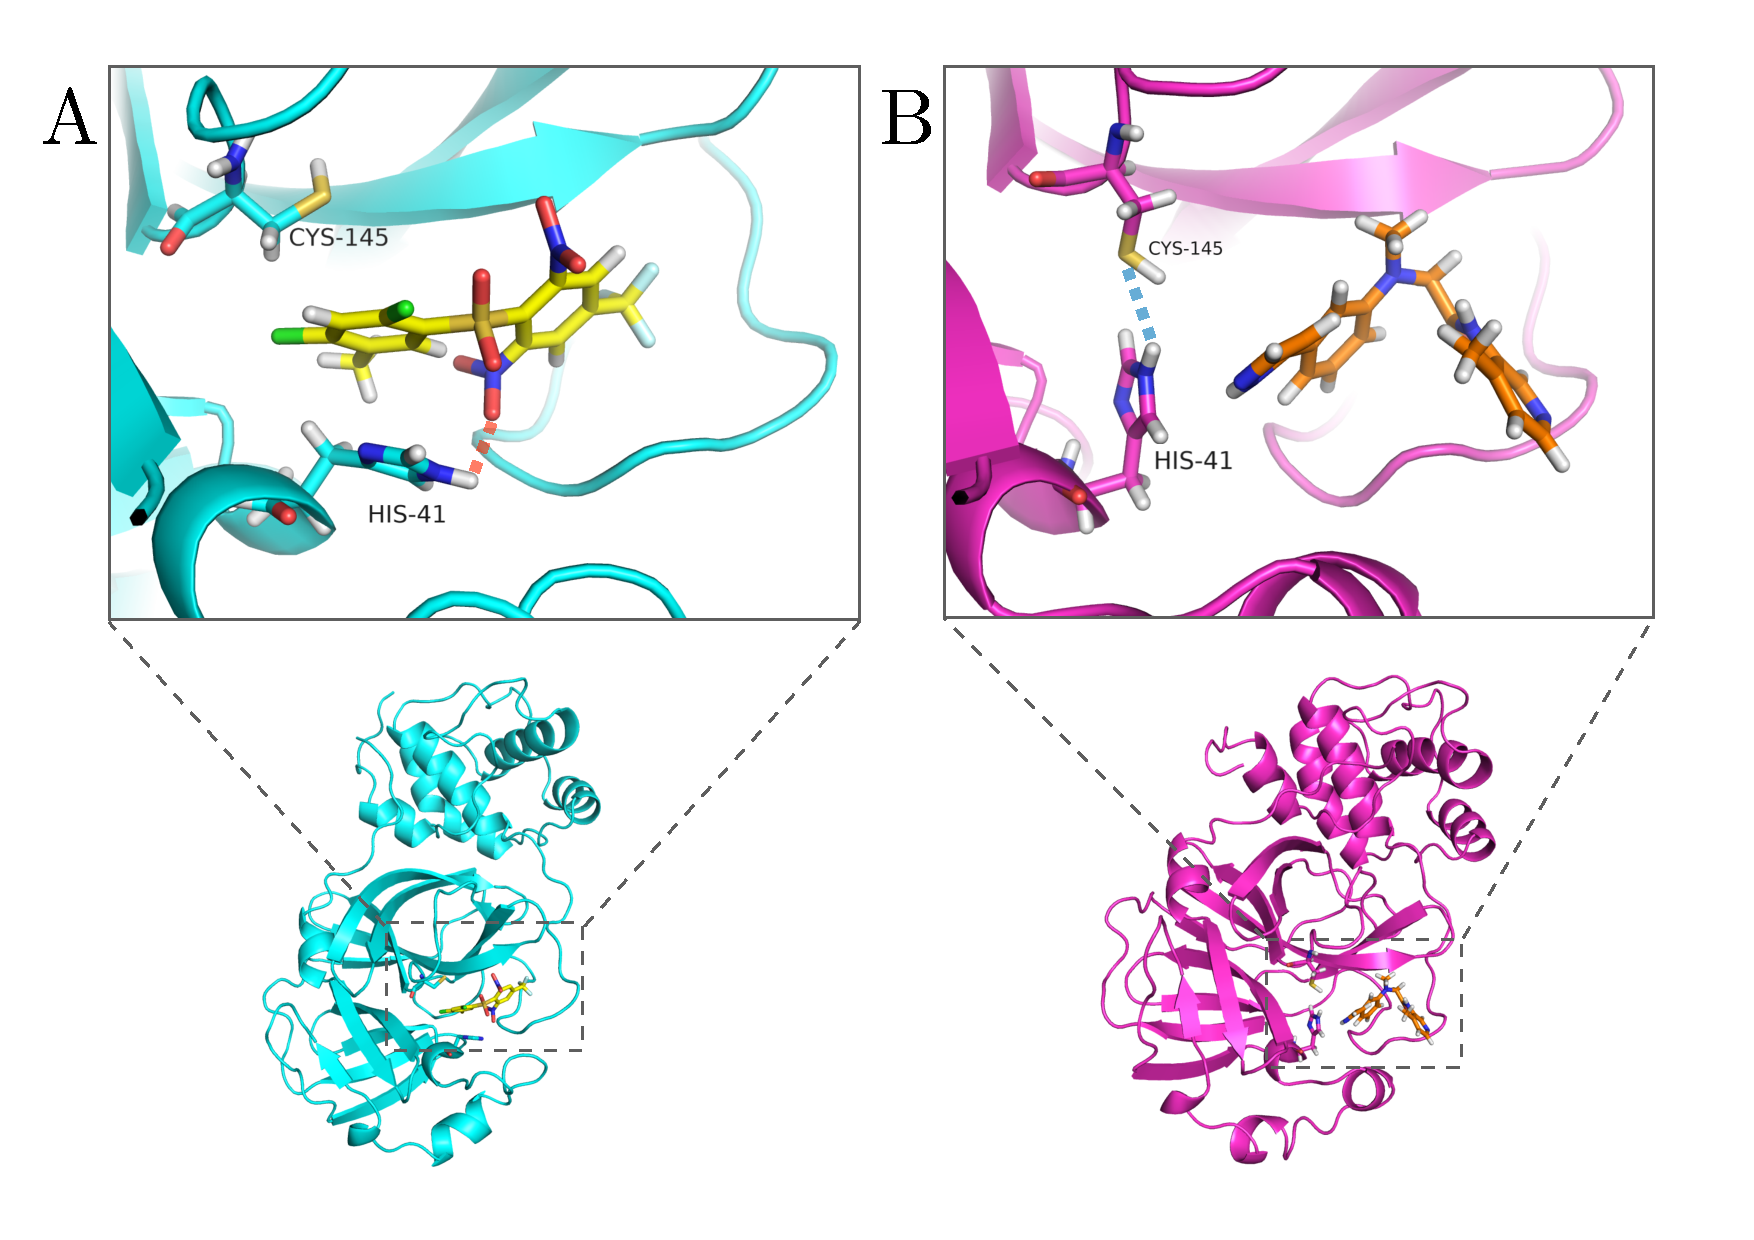
\includegraphics[width=\linewidth]{figures/side_by_side_labeled.pdf}
    \caption{The observed binding modes of (A) D3F (yellow) within the SARS-CoV-1  catalytic binding site (cyan), showing the disrupted catalytic dyad (``holo") and the strong D3F interaction with His41 (dashed red line) and (B) LIG (orange) within the SARS-CoV-2  catalytic binding site (pink) with a maintained catalytic dyad (``apo"). The dyad residues and their interactions (dashed blue line) are labeled His41 and Cys145.}
    \label{fig:bound_structures}
\end{figure}
\subsection{Generating the SARS-CoV-2  active state via His41 side chain reorientation}
%
The disruption of the catalytic dyad to promote ligand binding was further explored through the use of enhanced sampling simulations. The binding mode of D3F to SARS-CoV-1  indicates an ability to achieve inhibition of SARS-CoV-2  through promoting interactions with the His41 imidazole in the holo form. Metadynamics (MetaD) is herein employed with a bias potential over the \dihone dihedral of His41 in order to induce rotation of the His41 side chain imidazole group about the \dihtwo dihedral. The \dihtwo dihedral cannot be used as a CV due to an intrinsic conformational restriction, since the dihedral is part of the protein backbone. Instead, we have applied a bias to the \dihone dihedral torsion, which allows us to investigate the free rotational orientation of the His41 side chain imidazole (Fig.~\ref{fig:dihedrals}).\\
%
\begin{figure}
  \centering
  \begin{tabular}{@{}p{0.5\linewidth}@{\quad}p{0.5\linewidth}@{}}
    \subfigimg[width=\linewidth]{\large{\textbf{A} \quad $\mathbf{\xi_{1}}$ dihedral }}{chi1} &
    \subfigimg[width=\linewidth]{\large{\textbf{B} \quad $\mathbf{\xi_{2}^{backbone}}$ dihedral}}{chi2}
  \end{tabular}
  \caption{His41 imidazole side chain dihedrals. (A) \dihone dihedral used for construction of the MetaD bias. (B) \dihtwo dihedral considered within analysis of the performance of the bias and characterising the disassociation of His41 from Cys145.}
\label{fig:dihedrals}
\end{figure}

Ergodic sampling along the \dihone torsional CV space was achieved using MetaD simulations. The free energy surface with respect to the \dihone dihedral was calculated and is shown in (Fig.~\ref{fig:freeenergy_convergence}, top). This surface was used to verify metadynamics convergence by evaluating the relative free energy differences between pairs of free energy minima, which stabilised after 70 ns (Fig.~\ref{fig:freeenergy_convergence}, bottom).


\begin{figure}
    \centering
    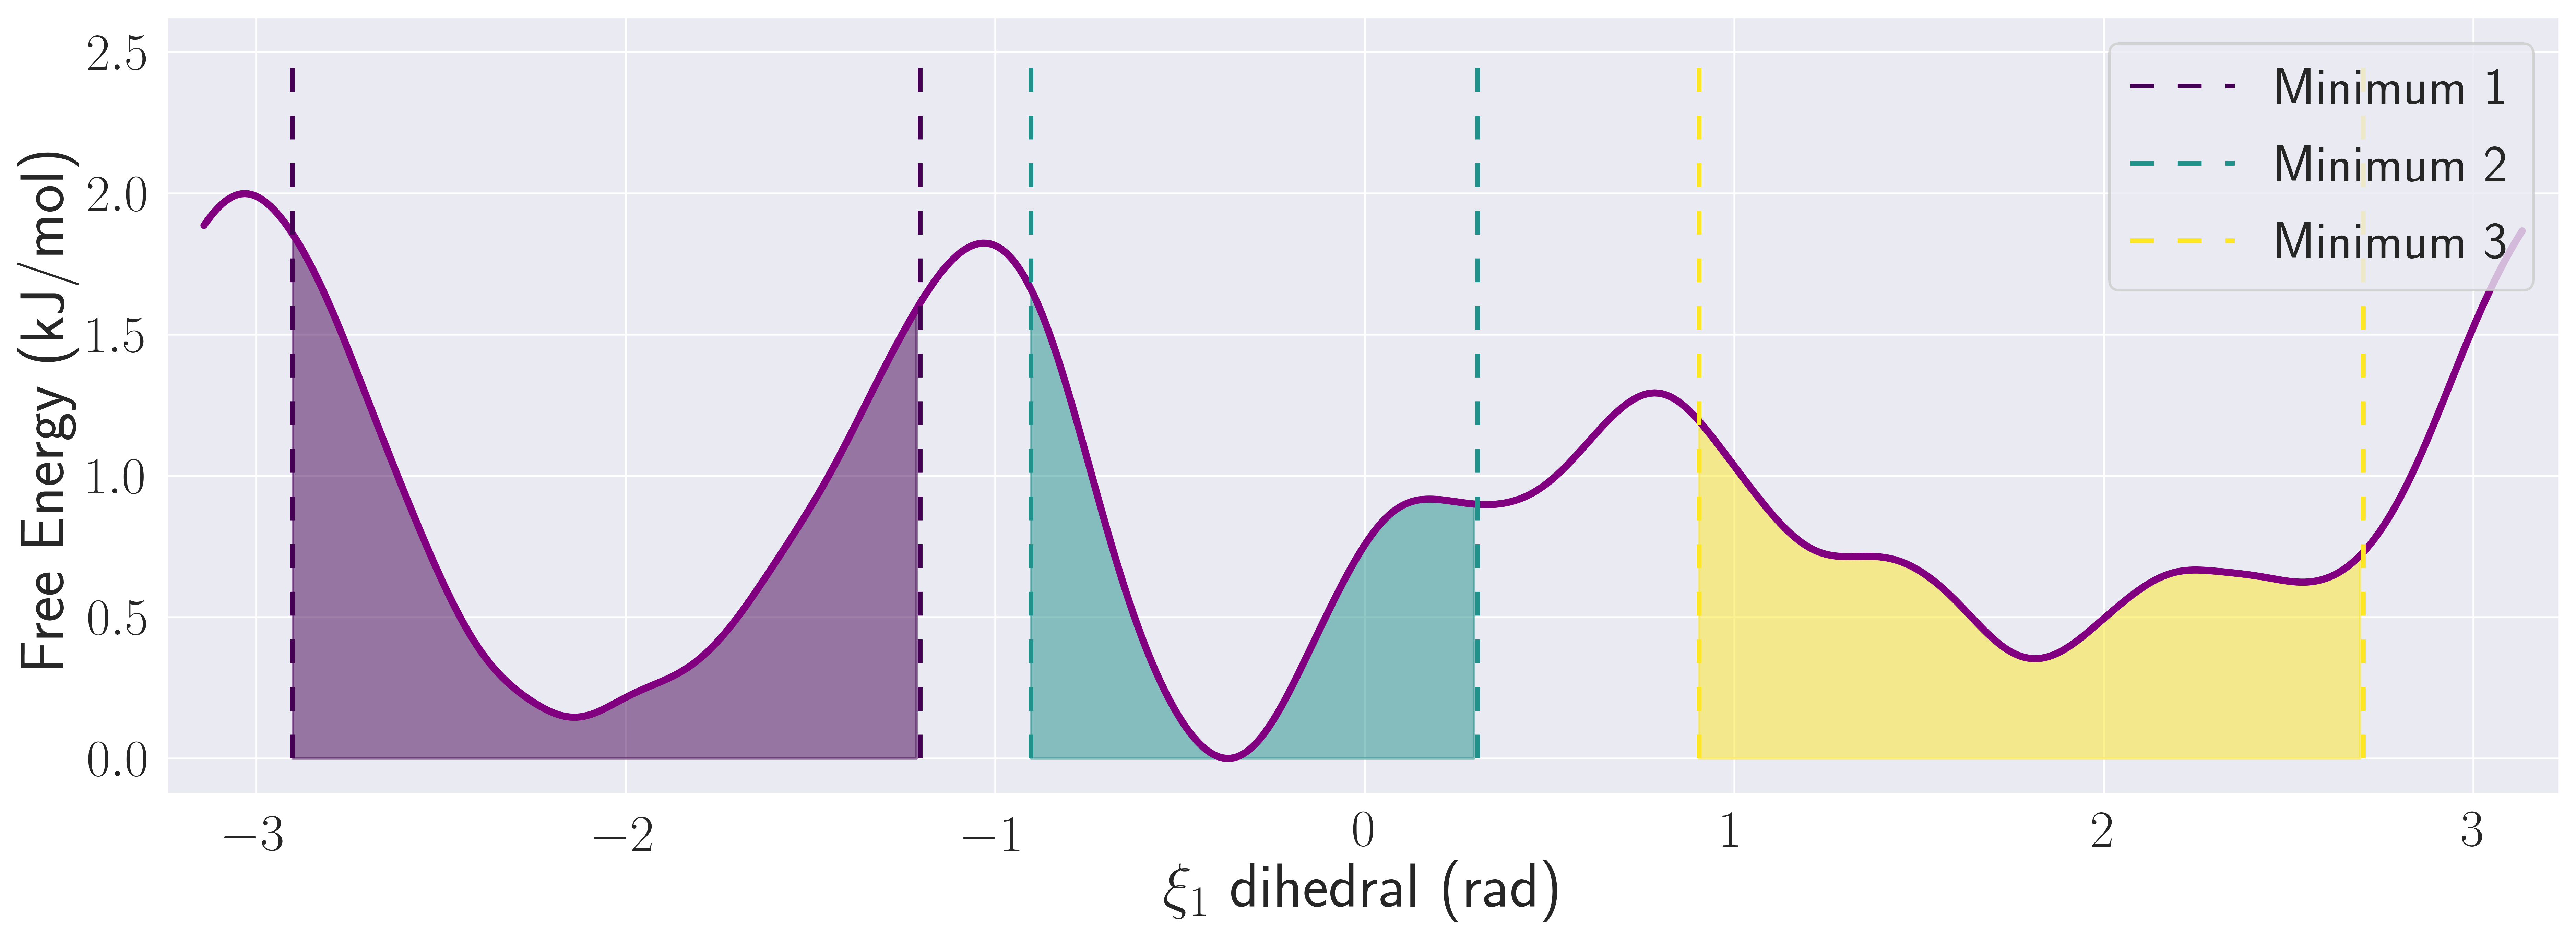
\includegraphics[width=\linewidth]{MetaDFES_segments.png}
    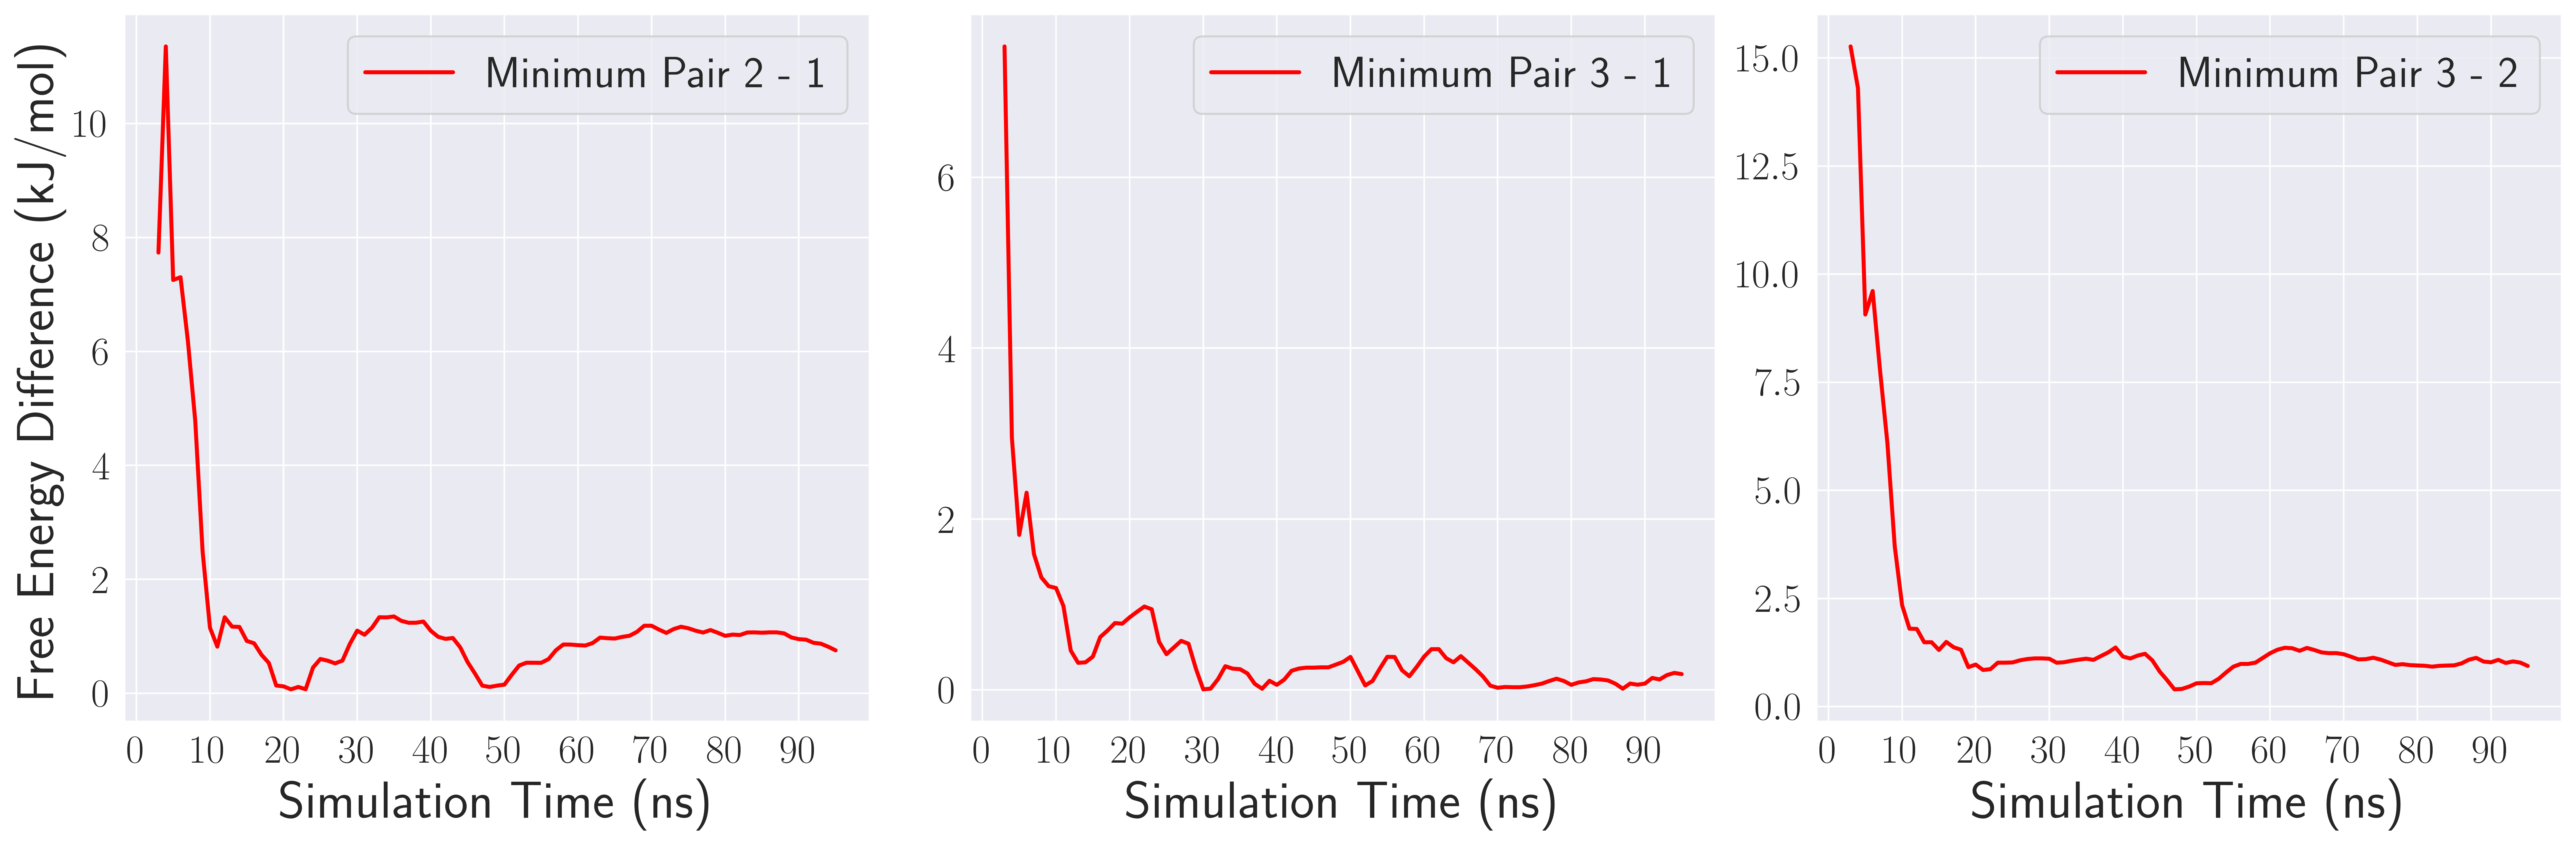
\includegraphics[width=\linewidth]{MetaDFES_convergence.png}
    \caption{\edit{Analysis of convergence of His41 imidazole dihedral MetaD bias potential. Potential of mean force (PMF) projected on the \dihone dihedral space of the bias potential. Relative free energy differences (in kJ/mol) were calculated between minima indicated by the dashed lines (top). Relative free energy difference between each pair of minima defined within the above PMF over the simulation time (bottom).}}
    \label{fig:freeenergy_convergence}
\end{figure}


\subsection{ catalytic dyad conformational changes}

In order to verify that our choice of CV of \dihone torsion couples to and changes the degree of \dihtwo torsion, we compare the probability densities found from our MetaD simulation to the probability distributions observed in our co-solvent MD simulations of LIG-SARS-CoV-2 and the D3F-SARS-CoV-1, which we use as the ``apo" (closed conformation) and ``holo" (open conformation) states, respectively. In (Fig.~\ref{fig:1Dim_PDF}A), the MetaD probability distribution clearly samples both ``apo" and ``holo" states. In (Fig.~\ref{fig:1Dim_PDF}B), this choice of \dihone torsion CV also biases the the catalytic dyad into an open state by orienting the His41 imidazole away from Cys145, measured through the (His41-N$_{\epsilon2}$)-(Cys145-S$_{\gamma}$) distance.\\

\begin{figure}
    \centering
    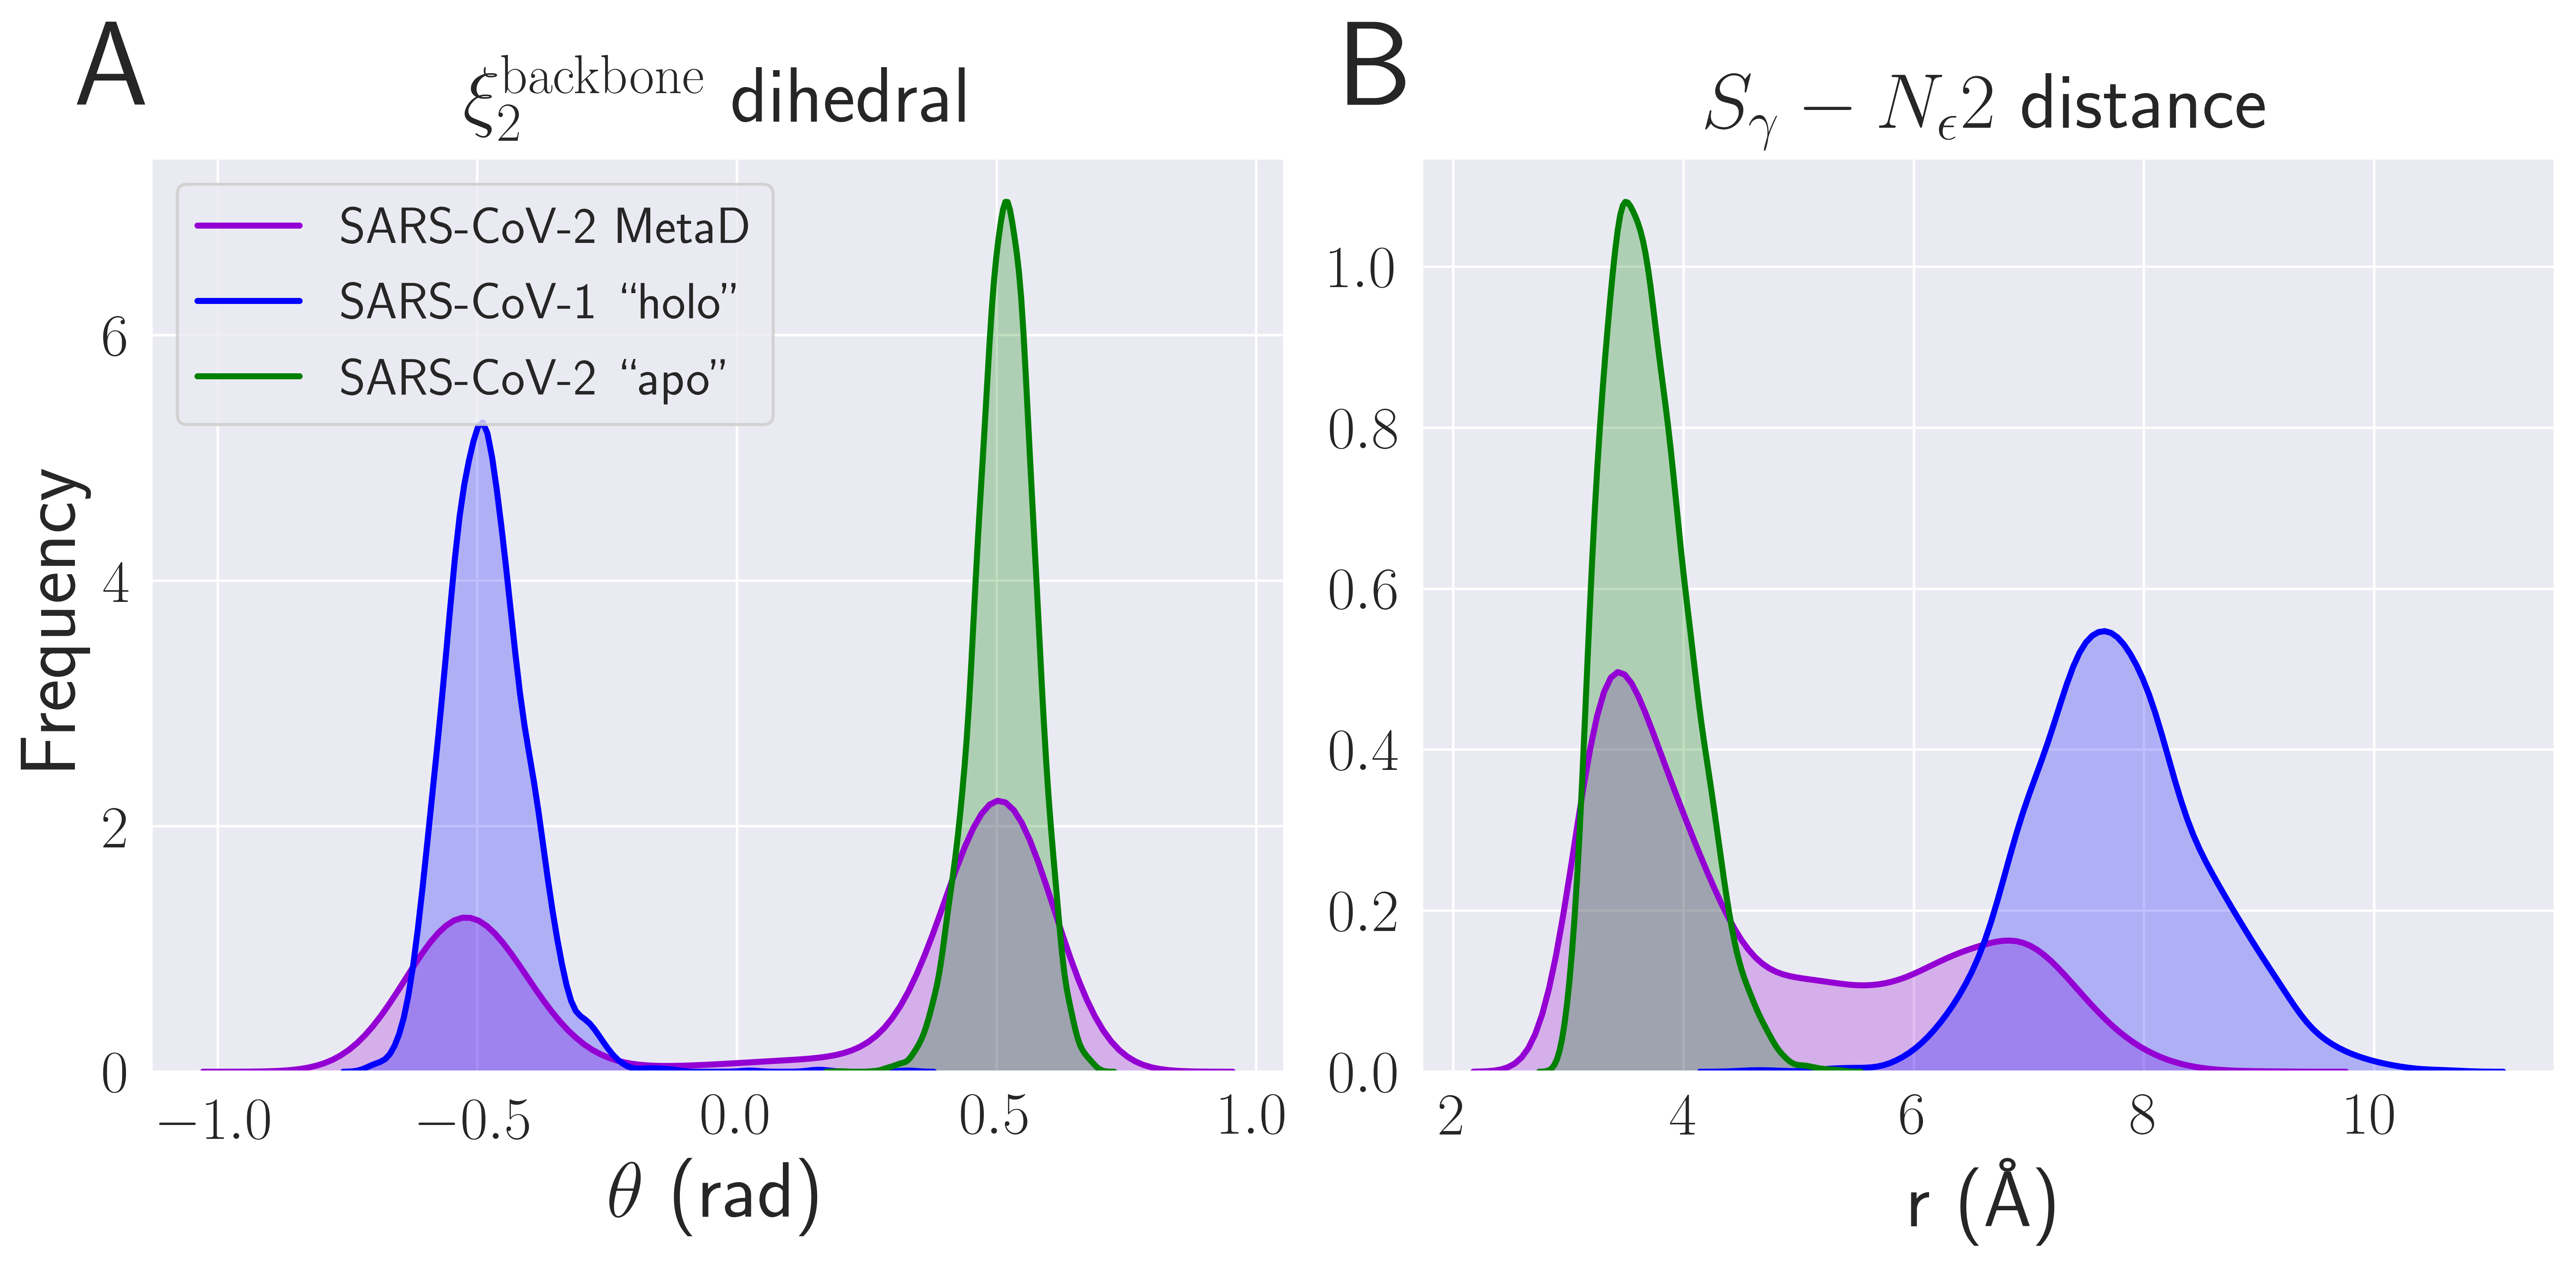
\includegraphics[width=0.8\linewidth]{MetaDPMF.png}
    \caption{1D probability density functions obtained from the co-solvent MD simulations of SARS-CoV-1 ``holo" (blue), SARS-CoV-2 ``apo" (green) and SARS-CoV-2 MetaD simulation (purple) over the (A) \dihtwo dihedral space and (B) (Cys145-S$_{\gamma}$)-(His41-N{$\epsilon$}) distance.} 
    \label{fig:1Dim_PDF}
\end{figure}

To demonstrate the interconnection of the \dihtwo torsion and (Cys145-S$_{\gamma}$)-(His41-N{$\epsilon$}) distance, we can represent the sampling of co-solvent MD simulations (``holo" - (Fig.~\ref{fig:2DPMF}A) and ``apo" - (Fig.~\ref{fig:2DPMF}C)) with the interchangeable MetaD sampling of both ``apo" and ``holo" states in a 2D space (Fig.~\ref{fig:2DPMF}B).  Comparing against the three density functions, it is noted that the region about \dihtwo = -0.5 rad overlaps with the ``holo" state, while the region about \dihtwo = 0.5 rad overlaps with the sampled density of the ``apo" in which the catalytic dyad remains intact throughout. This comparison allows for the characterisation of each of the respective regions in the metadynamics density function above to be considered as ``apo" and ``holo" conformational states (Fig.~\ref{fig:2DPMF}B).\\

In (Fig.~\ref{fig:2DPMF}B), the bimodal probability density in the 2D CV space includes points at shorter (Cys145-$S_{\gamma}$)--(His41-N{$\epsilon$}) distances at \dihtwo = -0.5 rad. This region indicates that, in the absence of a potent inhibitor, the ``holo" state cannot be stabilised by biased \dihone sampling alone. As such, the dyad will reorient to maintain the Cys145-His41 side chain interaction.\\

\begin{figure}[ht!]
  \centering
    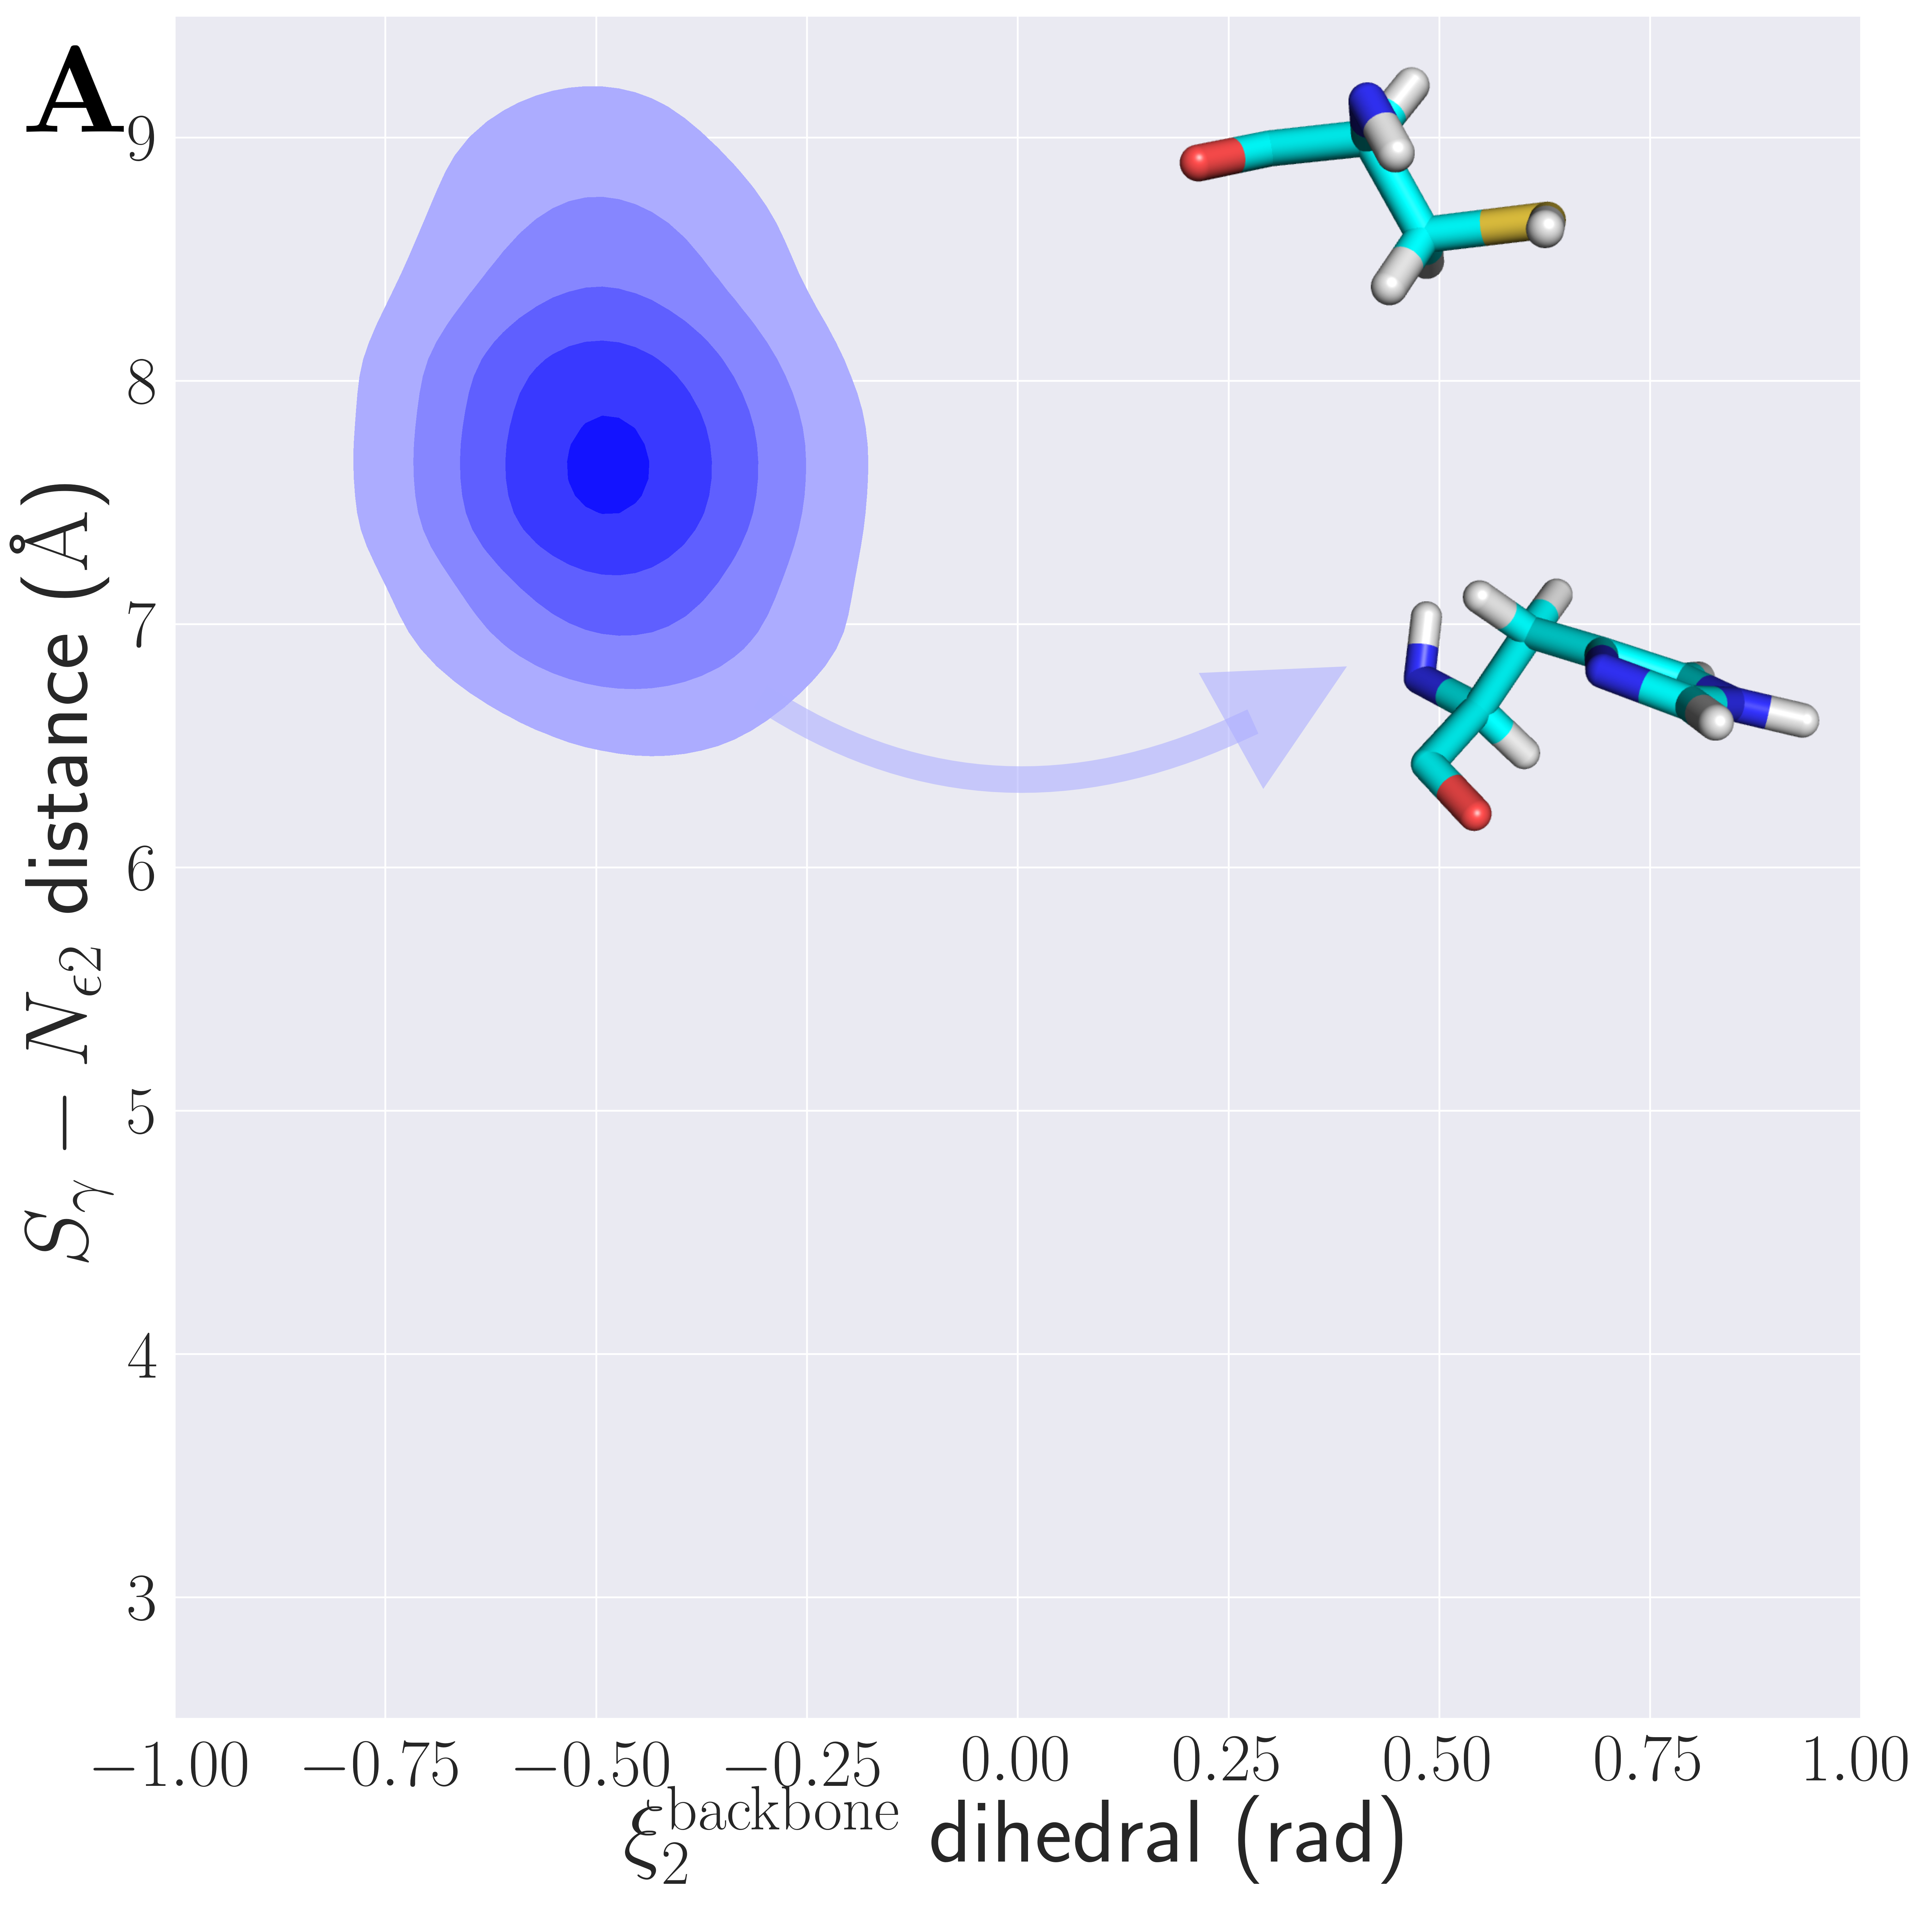
\includegraphics[width=0.3\linewidth]{HOLO_2DPMF.png}
    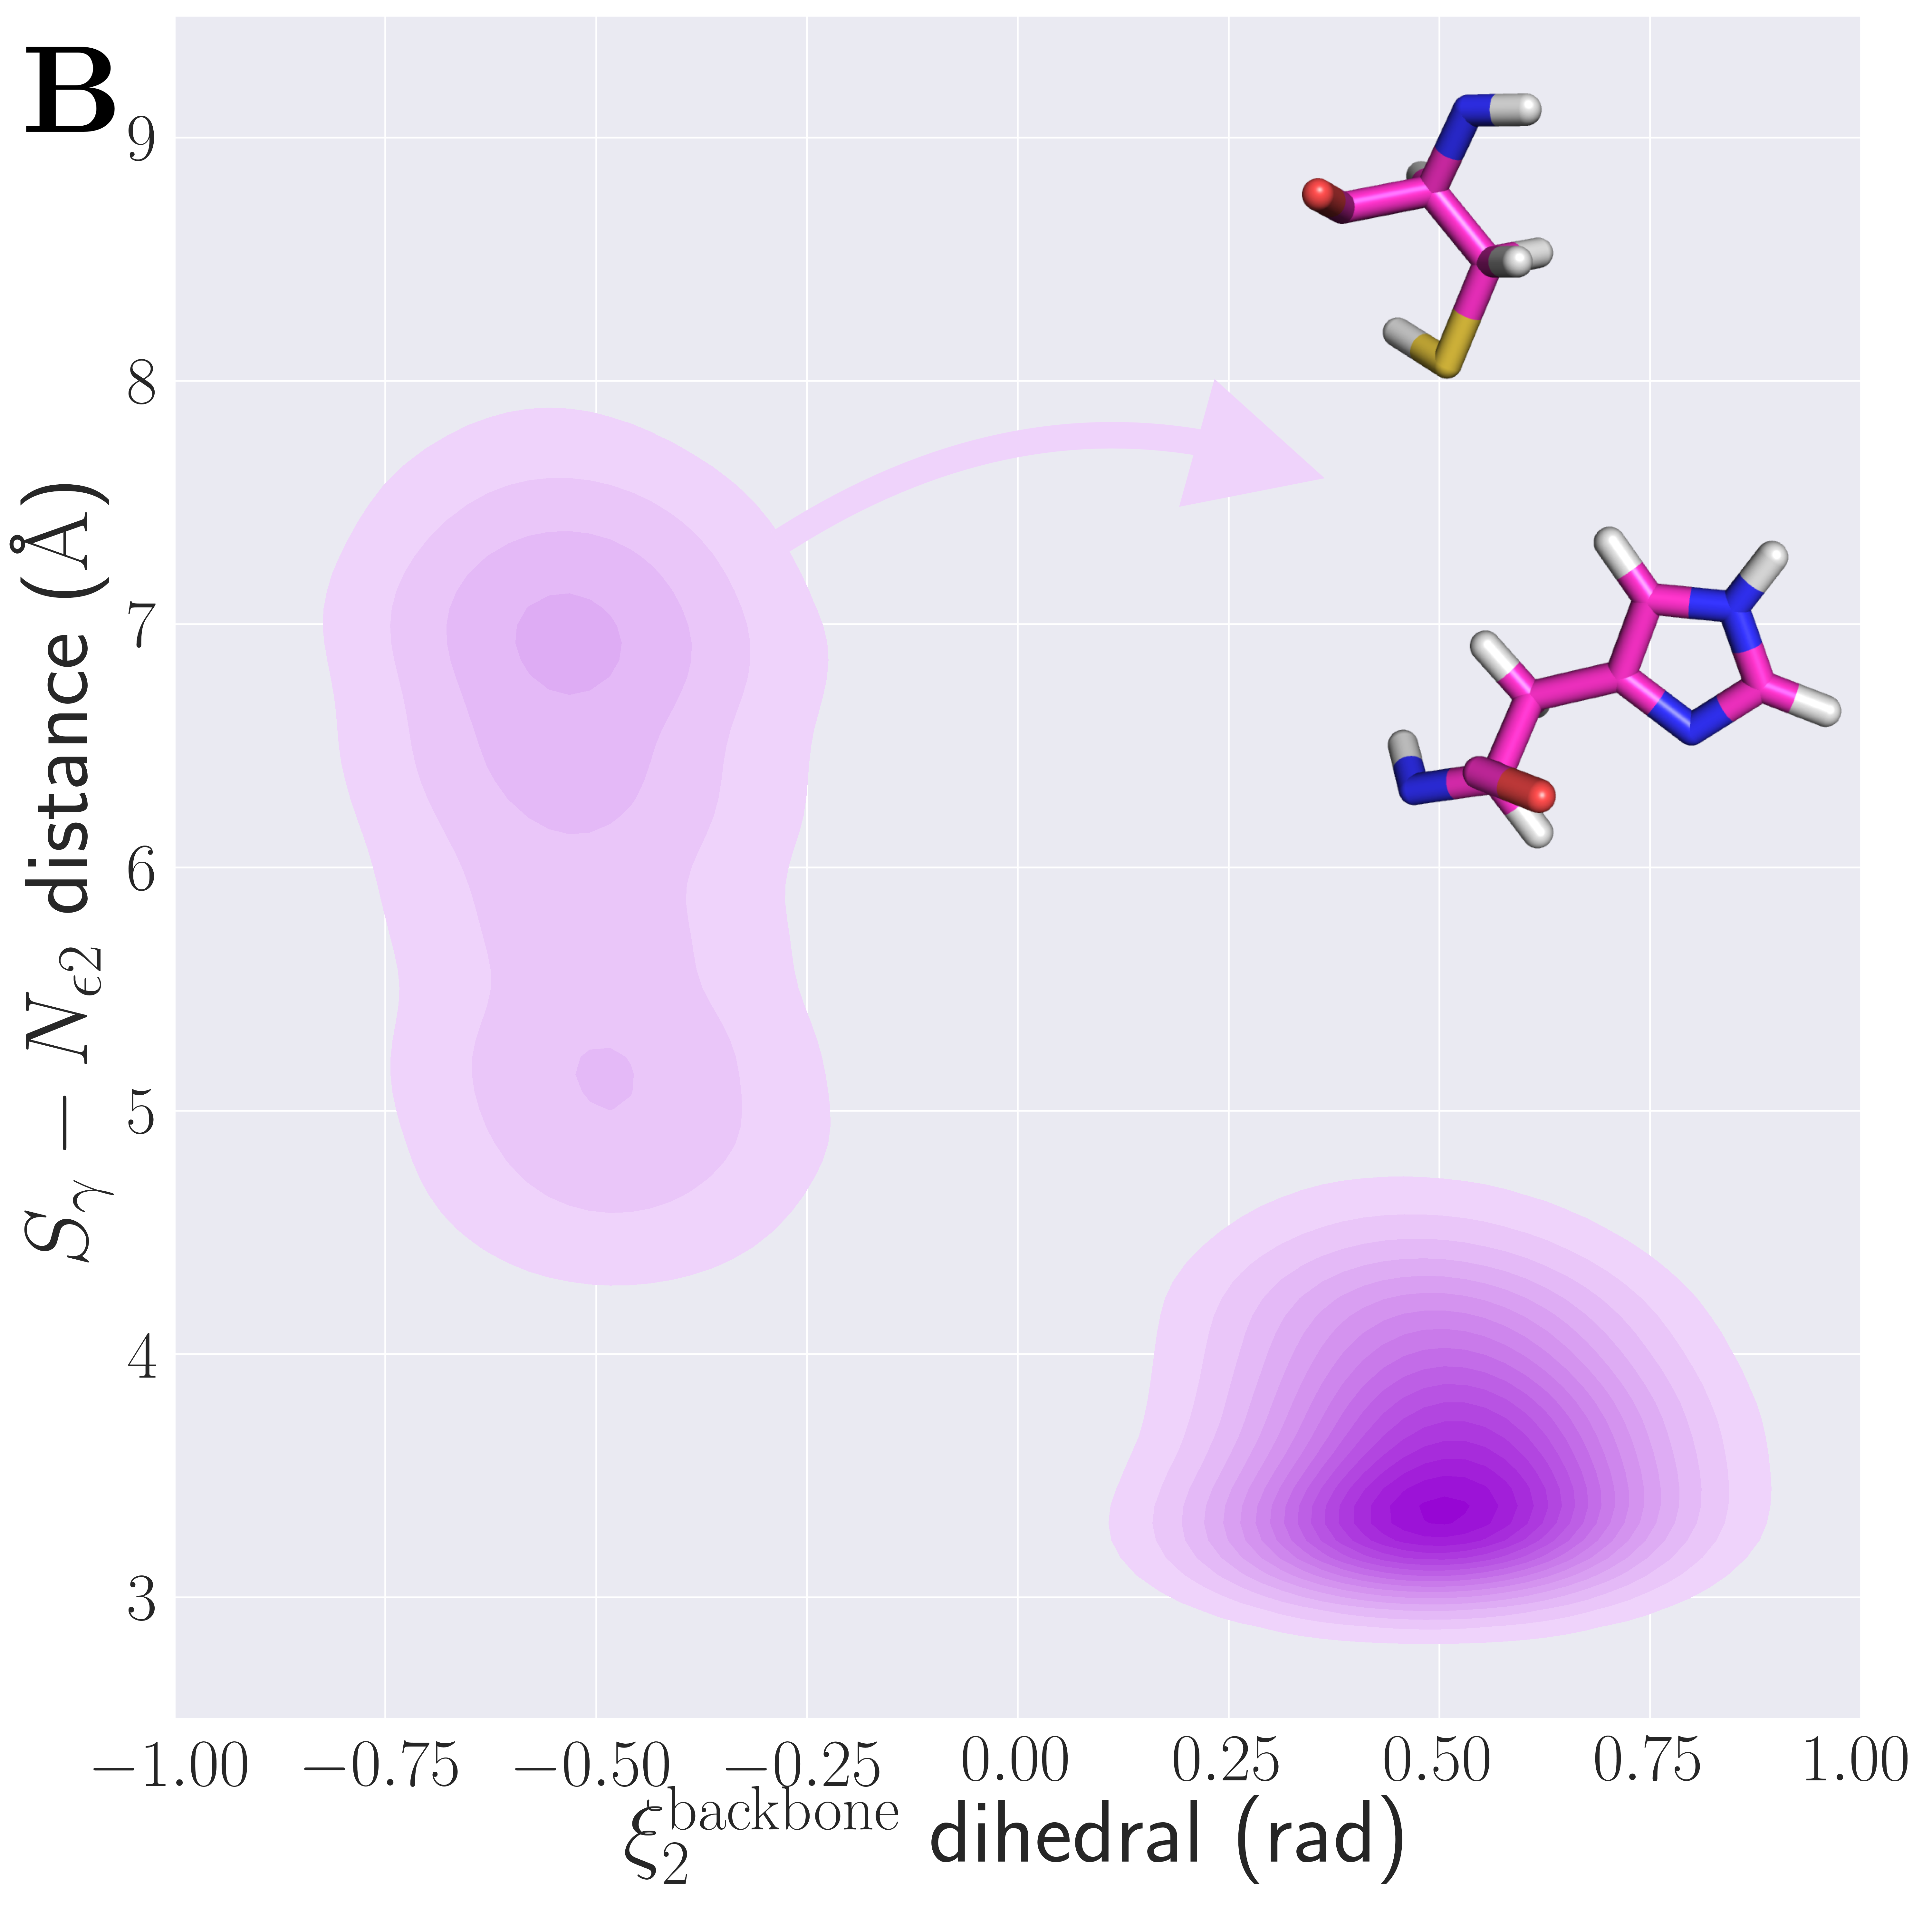
\includegraphics[width=0.3\linewidth]{MetaD_2DPMF.png}
    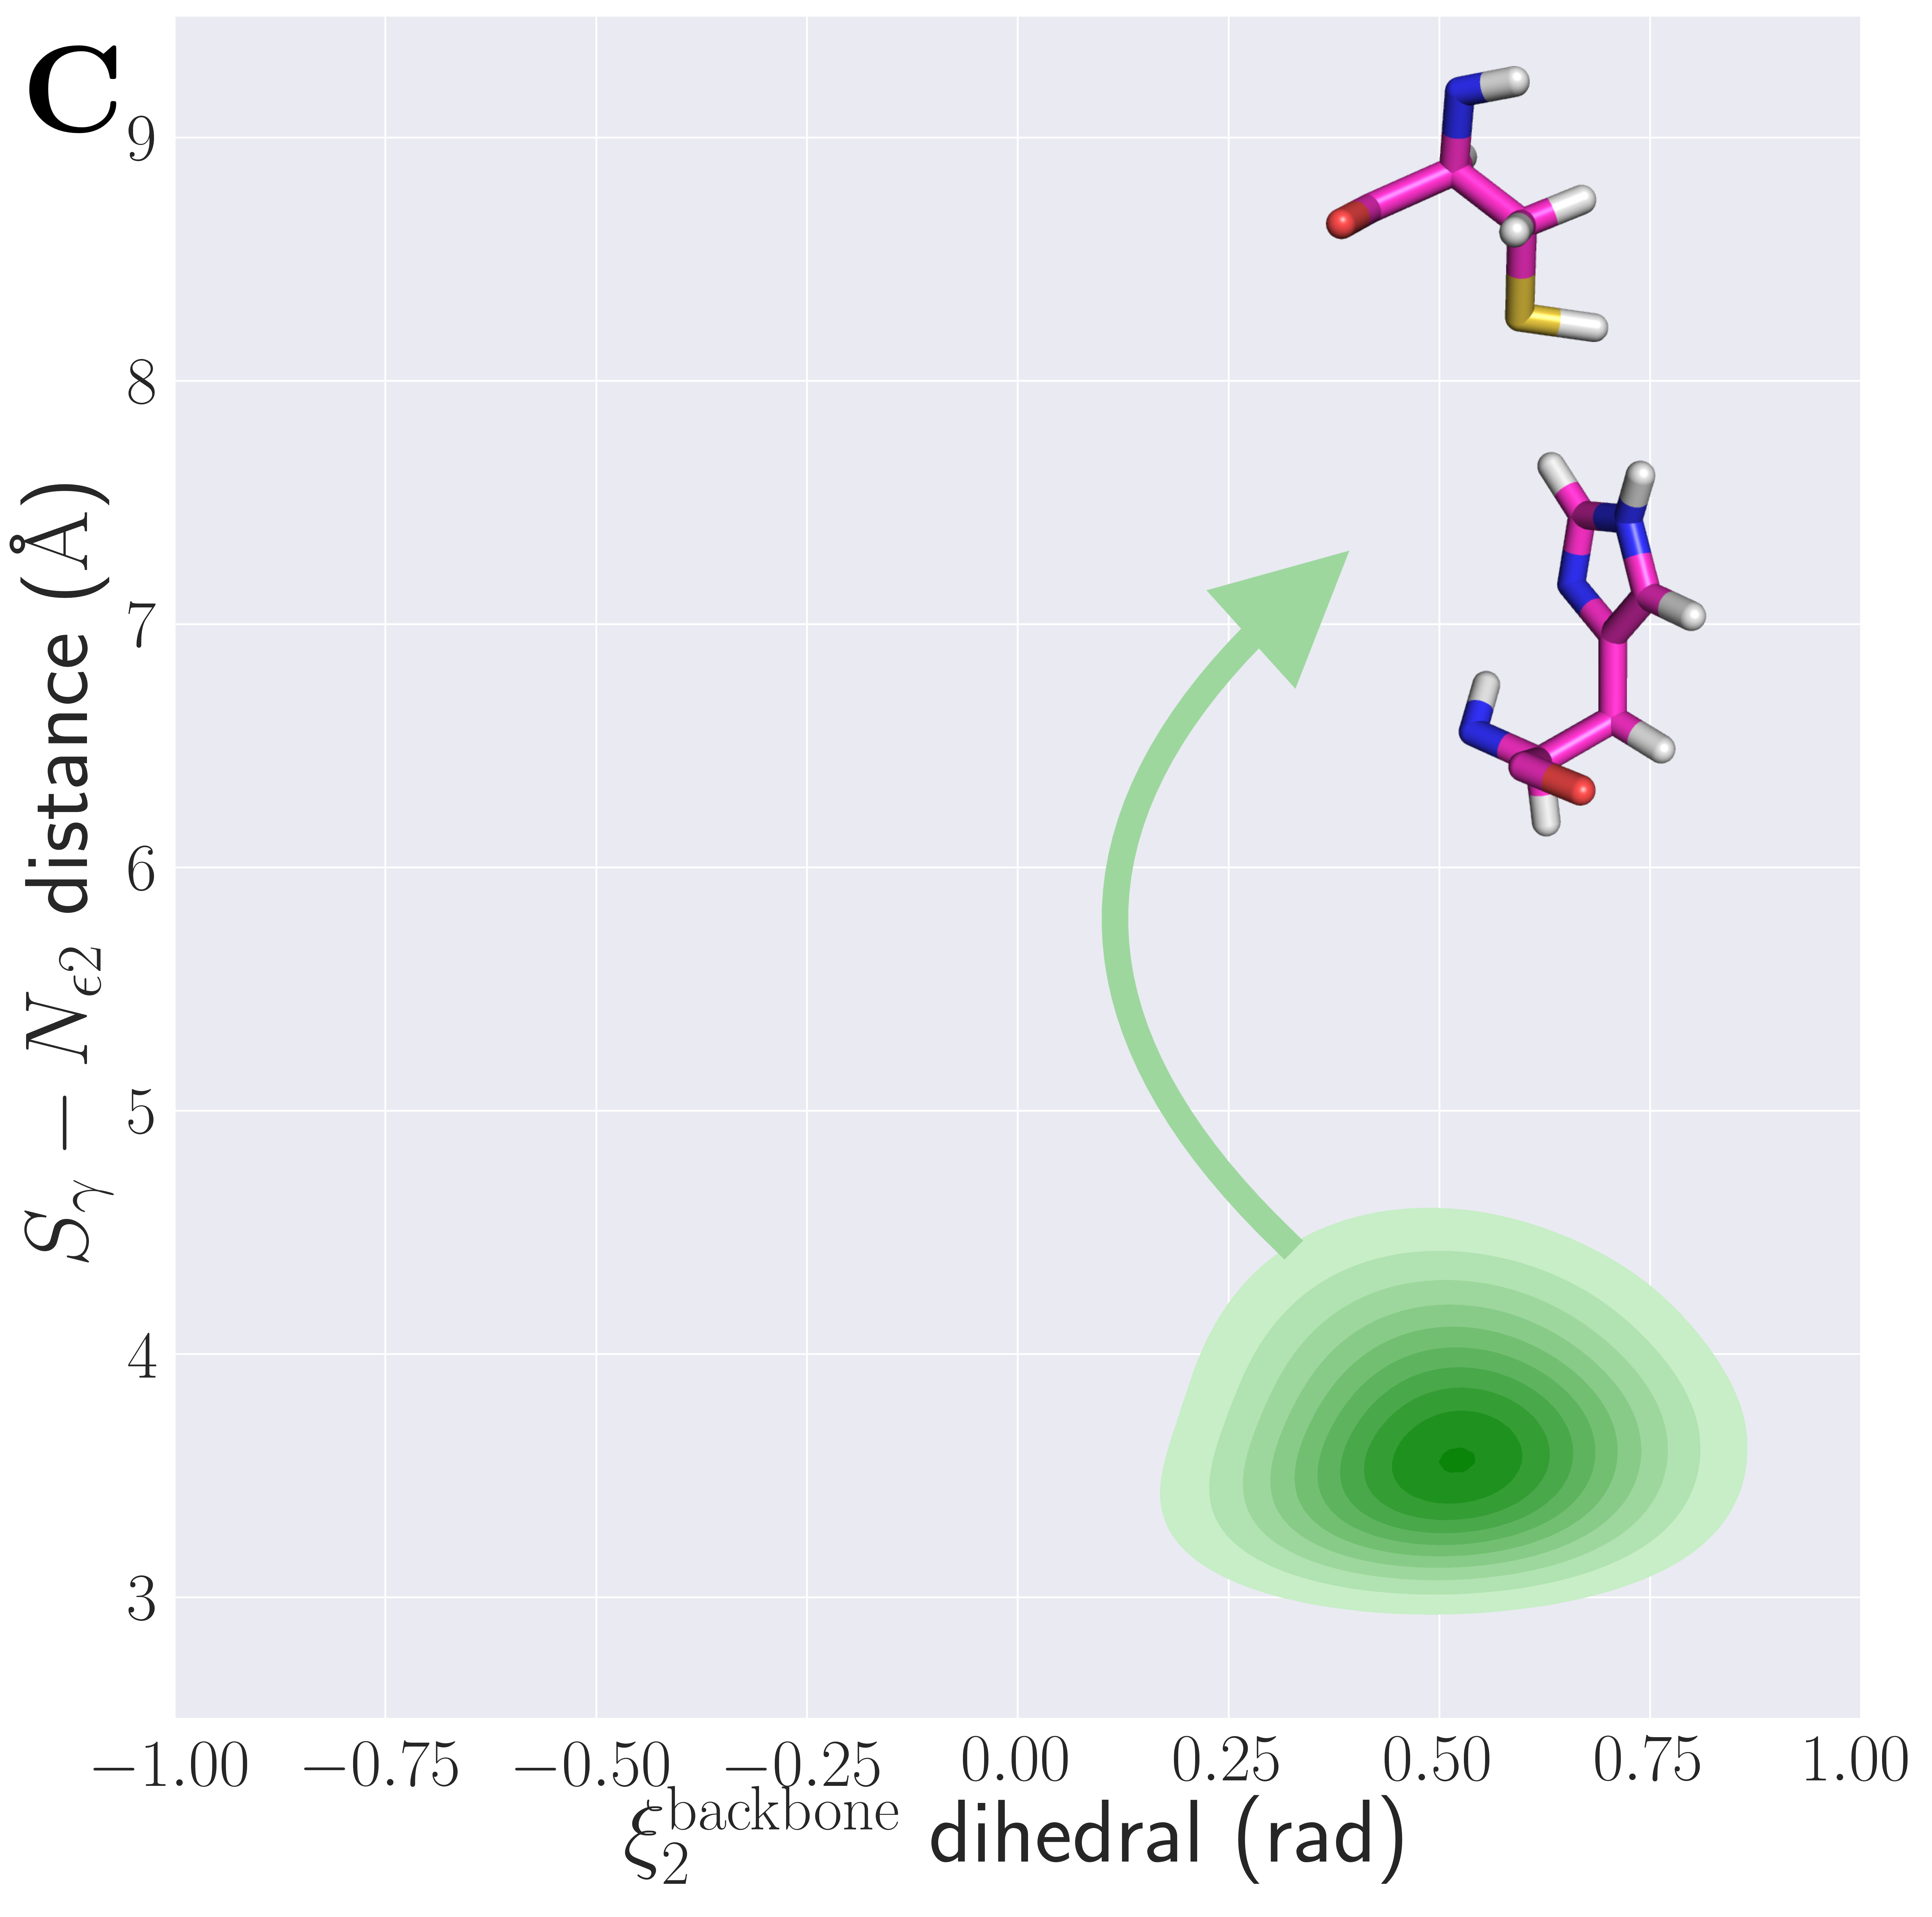
\includegraphics[width=0.3\linewidth]{APO_2DPMF.png}
  \caption{Probability density functions of the (A) SARS-CoV-1 ``holo" , (B) SARS-CoV-2 MetaD (inset showing MetaD ``holo") and (C) SARS-CoV-2 ``apo" MD simulation defined within a 2D CV space of the His41 \dihtwo dihedral and the (Cys145-$S_{\gamma}$)-(His41-N{$\epsilon$}) atomic distance.}
  \label{fig:2DPMF}
\end{figure}


To confirm that the choice of a \dihone bias samples the ``apo"--``holo" transition, the time-dependent behaviour of both the \dihtwo dihedral and the (Cys145-$S_{\gamma}$)-(His41-N{$\epsilon$}) distance was evaluated using K-means clustering.\cite{scikit-learn} Three distinct clusters were found (Fig.~\ref{fig:2DAveragePMF}) corresponding to the ``apo" conformation (\dihtwo = 0.5 rad) , ``holo" conformation (\dihtwo = -0.5 rad) and transition region. The time dependent behaviour of \dihtwo dihedral and (Cys145-$S_{\gamma}$)-(His41-N{$\epsilon$}) distance show the choice of CV freely samples the reversible ``apo"--``holo" transition throughout the 100 ns trajectory.\\

\begin{figure}[!ht]
    \centering
    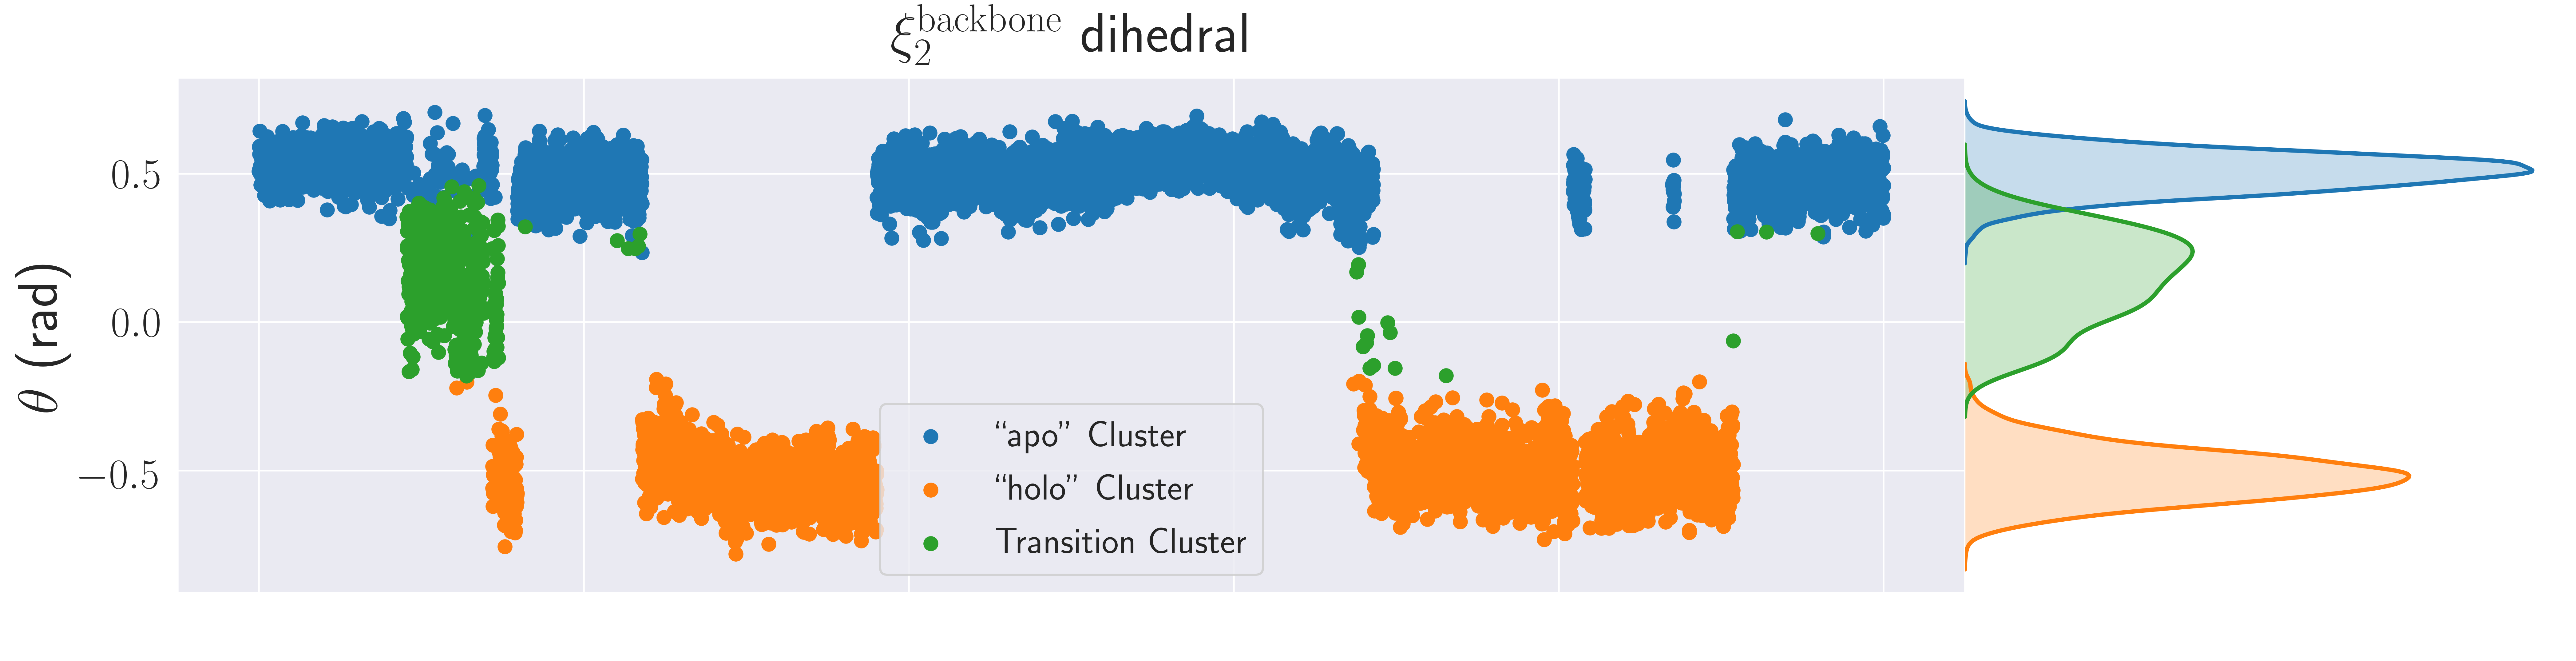
\includegraphics[width=\linewidth]{KMeansVsTime_0.png}
    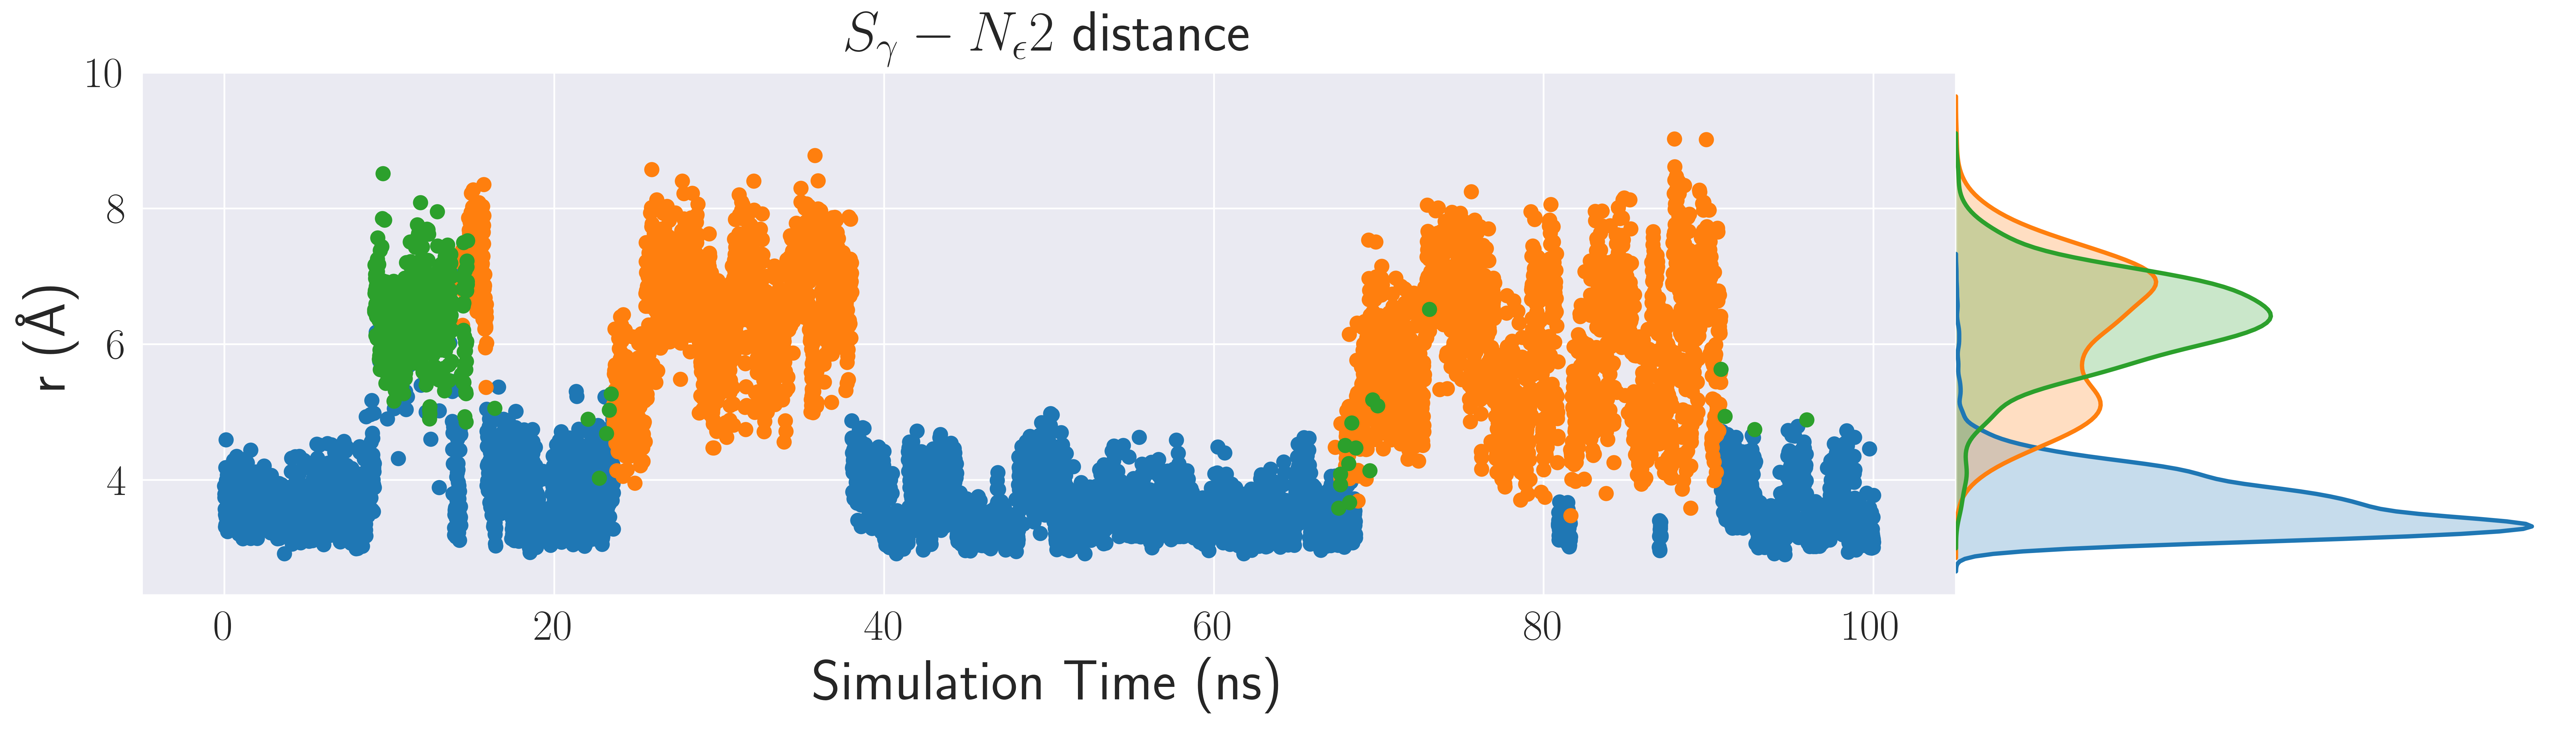
\includegraphics[width=\linewidth]{KMeansVsTime_1.png}
    \caption{\edit{Time evolution of the MetaD simulation trajectory and the associated cluster identity of points with respect to the His41 \dihtwo dihedral (top) and the (Cys145-S$_{\gamma}$)-(His41-N{$\epsilon$}) distance (bottom).}}
    \label{fig:2DAveragePMF}
\end{figure}

\subsection{ free energy surfaces}

In order to verify the reproducibility of the constructed bias, four replicas of the MetaD simulation were performed until convergence was observed in each. The free energy profiles obtained in each of the replicas show agreement, with deviation from the average free energy values observed chiefly at the transition states and at the minimum at \dihone = 1.9 rad. The deviation at this minimum is due to the corresponding state being sparsely sampled in all replicas compared to the other system states as a result of the high free energy barrier restricting sampling from other observed minima (Fig.~\ref{fig:AverageFES}).\\

\begin{figure}[!ht]
    \centering
    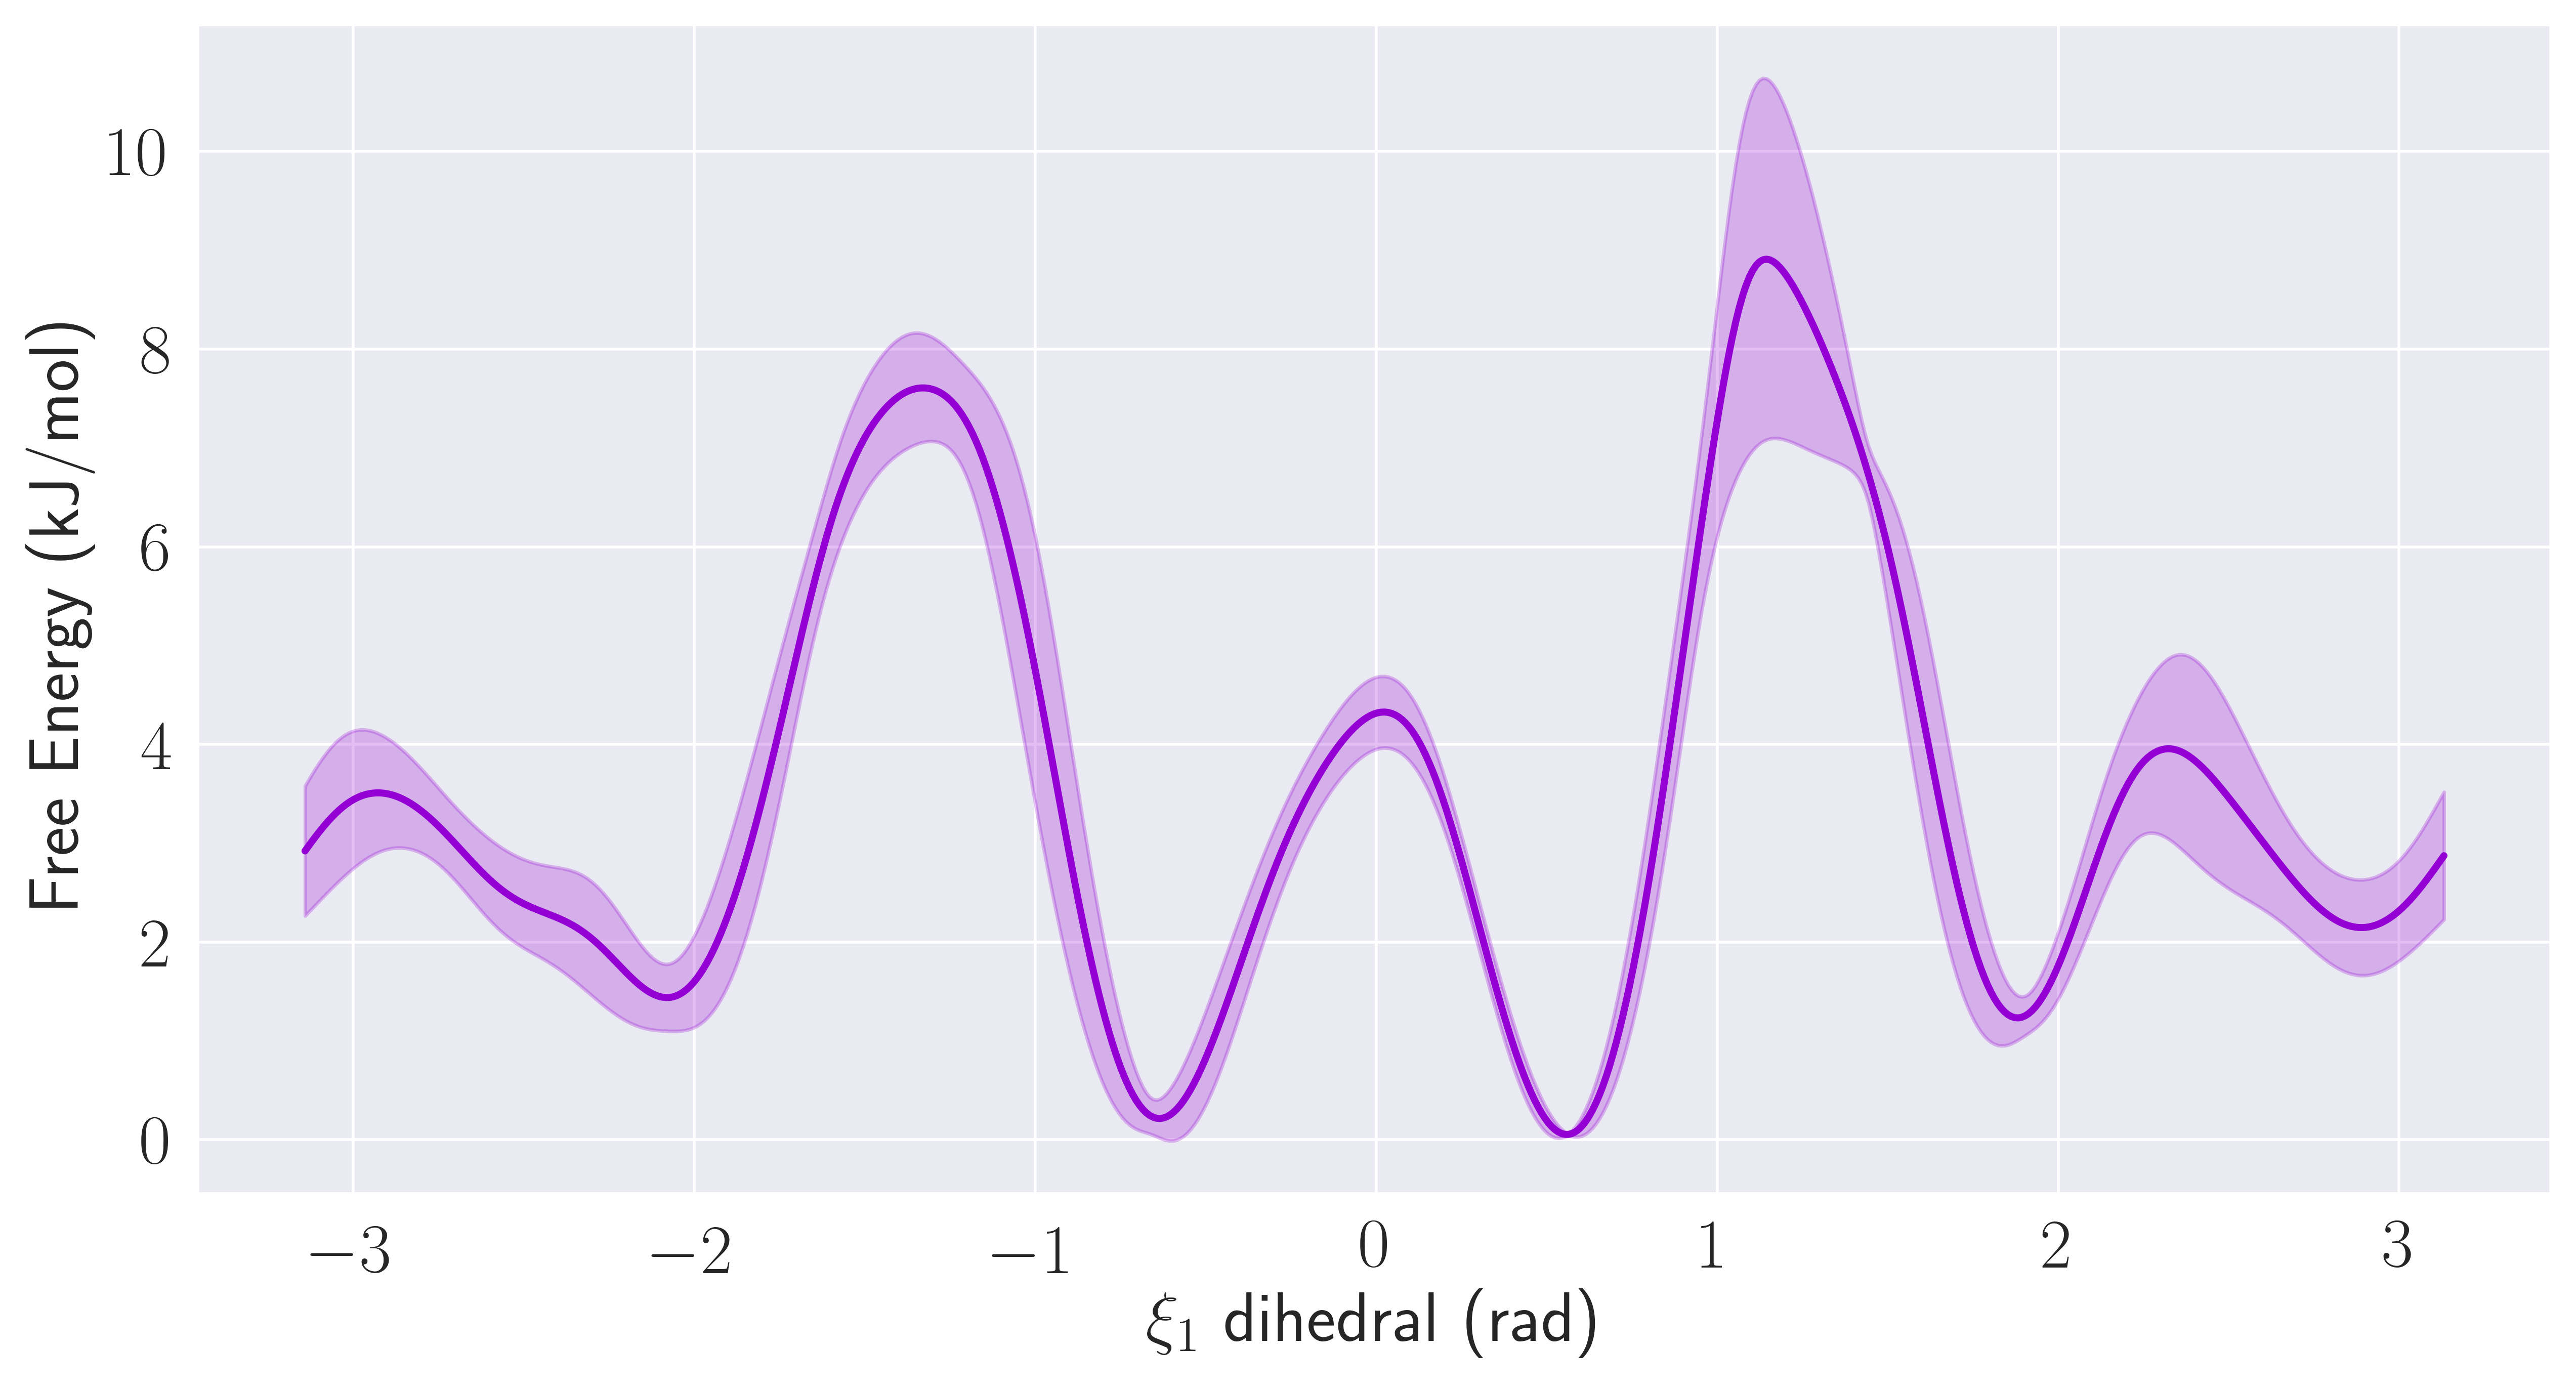
\includegraphics[width=\linewidth]{AverageFES_4Reps.png}
    \caption{\edit{Mean free energy surface obtained over 4 replicas of His41 torsional metadynamics defined within the \dihone dihedral space. The shaded region corresponds to the standard deviation about each free energy point calculated over the set of replicas.}}
    \label{fig:AverageFES}
\end{figure}

As convergence of the bias was observed for all four replicas, it can be assumed that any sampling beyond the point of convergence is within the desired thermodynamic ensemble. Thus, the mean free energy surface with respect to the His41 \dihtwo dihedral over the 4 replicas was computed (Fig \ref{fig:1DPMFAll_Dihtwo}). The mean surface is bimodal, with positions of the minima at 0.5 and -0.5 rad corresponding the the sampled ``apo" and ``holo" states of the SARS-CoV-2  catalytic dyad, respectively. The ``apo"-``holo" relative free energy difference of $4.2 \pm 1.9$ kJ/mol ($1.0 \pm 0.5$ kcal/mol) indicates that the ``holo" state is less energetically stable than the ``apo" state in the absence of any ligands interacting with His41. Considering this free energy difference between states and the high free energy barrier ($15.0 \pm 1.3$ kJ/mol / $3.6 \pm 0.3$ kcal/mol) between them, it can be assumed that the dyad ``apo"--``holo" transition is unlikely to be sampled using unbiased conventional MD simulations alone.\\

The free energy surface of SARS-CoV-1 ``holo" (dashed blue line) was computed from the reference simulation of the D3F-SARS-CoV-1  complex using population analysis (Fig.~\ref{fig:1DPMFAll_Dihtwo}). This surface is used as a reference state to compare against the mean MetaD free energy surface as the ``holo" state. The SARS-CoV-1 ``holo" conformation is more energetically stable than the SARS-CoV-2 MetaD surface ``holo" minimum by approximately $4.2 \pm 1.9$ kJ/mol ($1.0 \pm 0.5$ kcal/mol). This energy difference highlights how the energetic penalty associated with dyad disruption in the ``apo"--``holo" transition may be recovered by ligand interactions in the active site. \edit{All MetaD replicas yielded sampling of the two rotamers of His41 about the backbone dihedral. The larger error about the ``dyad disrupted" conformation at -0.5 rad (Fig.~\ref{fig:1DPMFAll_Dihtwo}) is due to sampling with a ligand-free active site for \!, meaning that less stable conformation isn't stabilised by ligand interactions unlike the case of D3F binding.}\\

\begin{figure}[!ht]
    \centering
    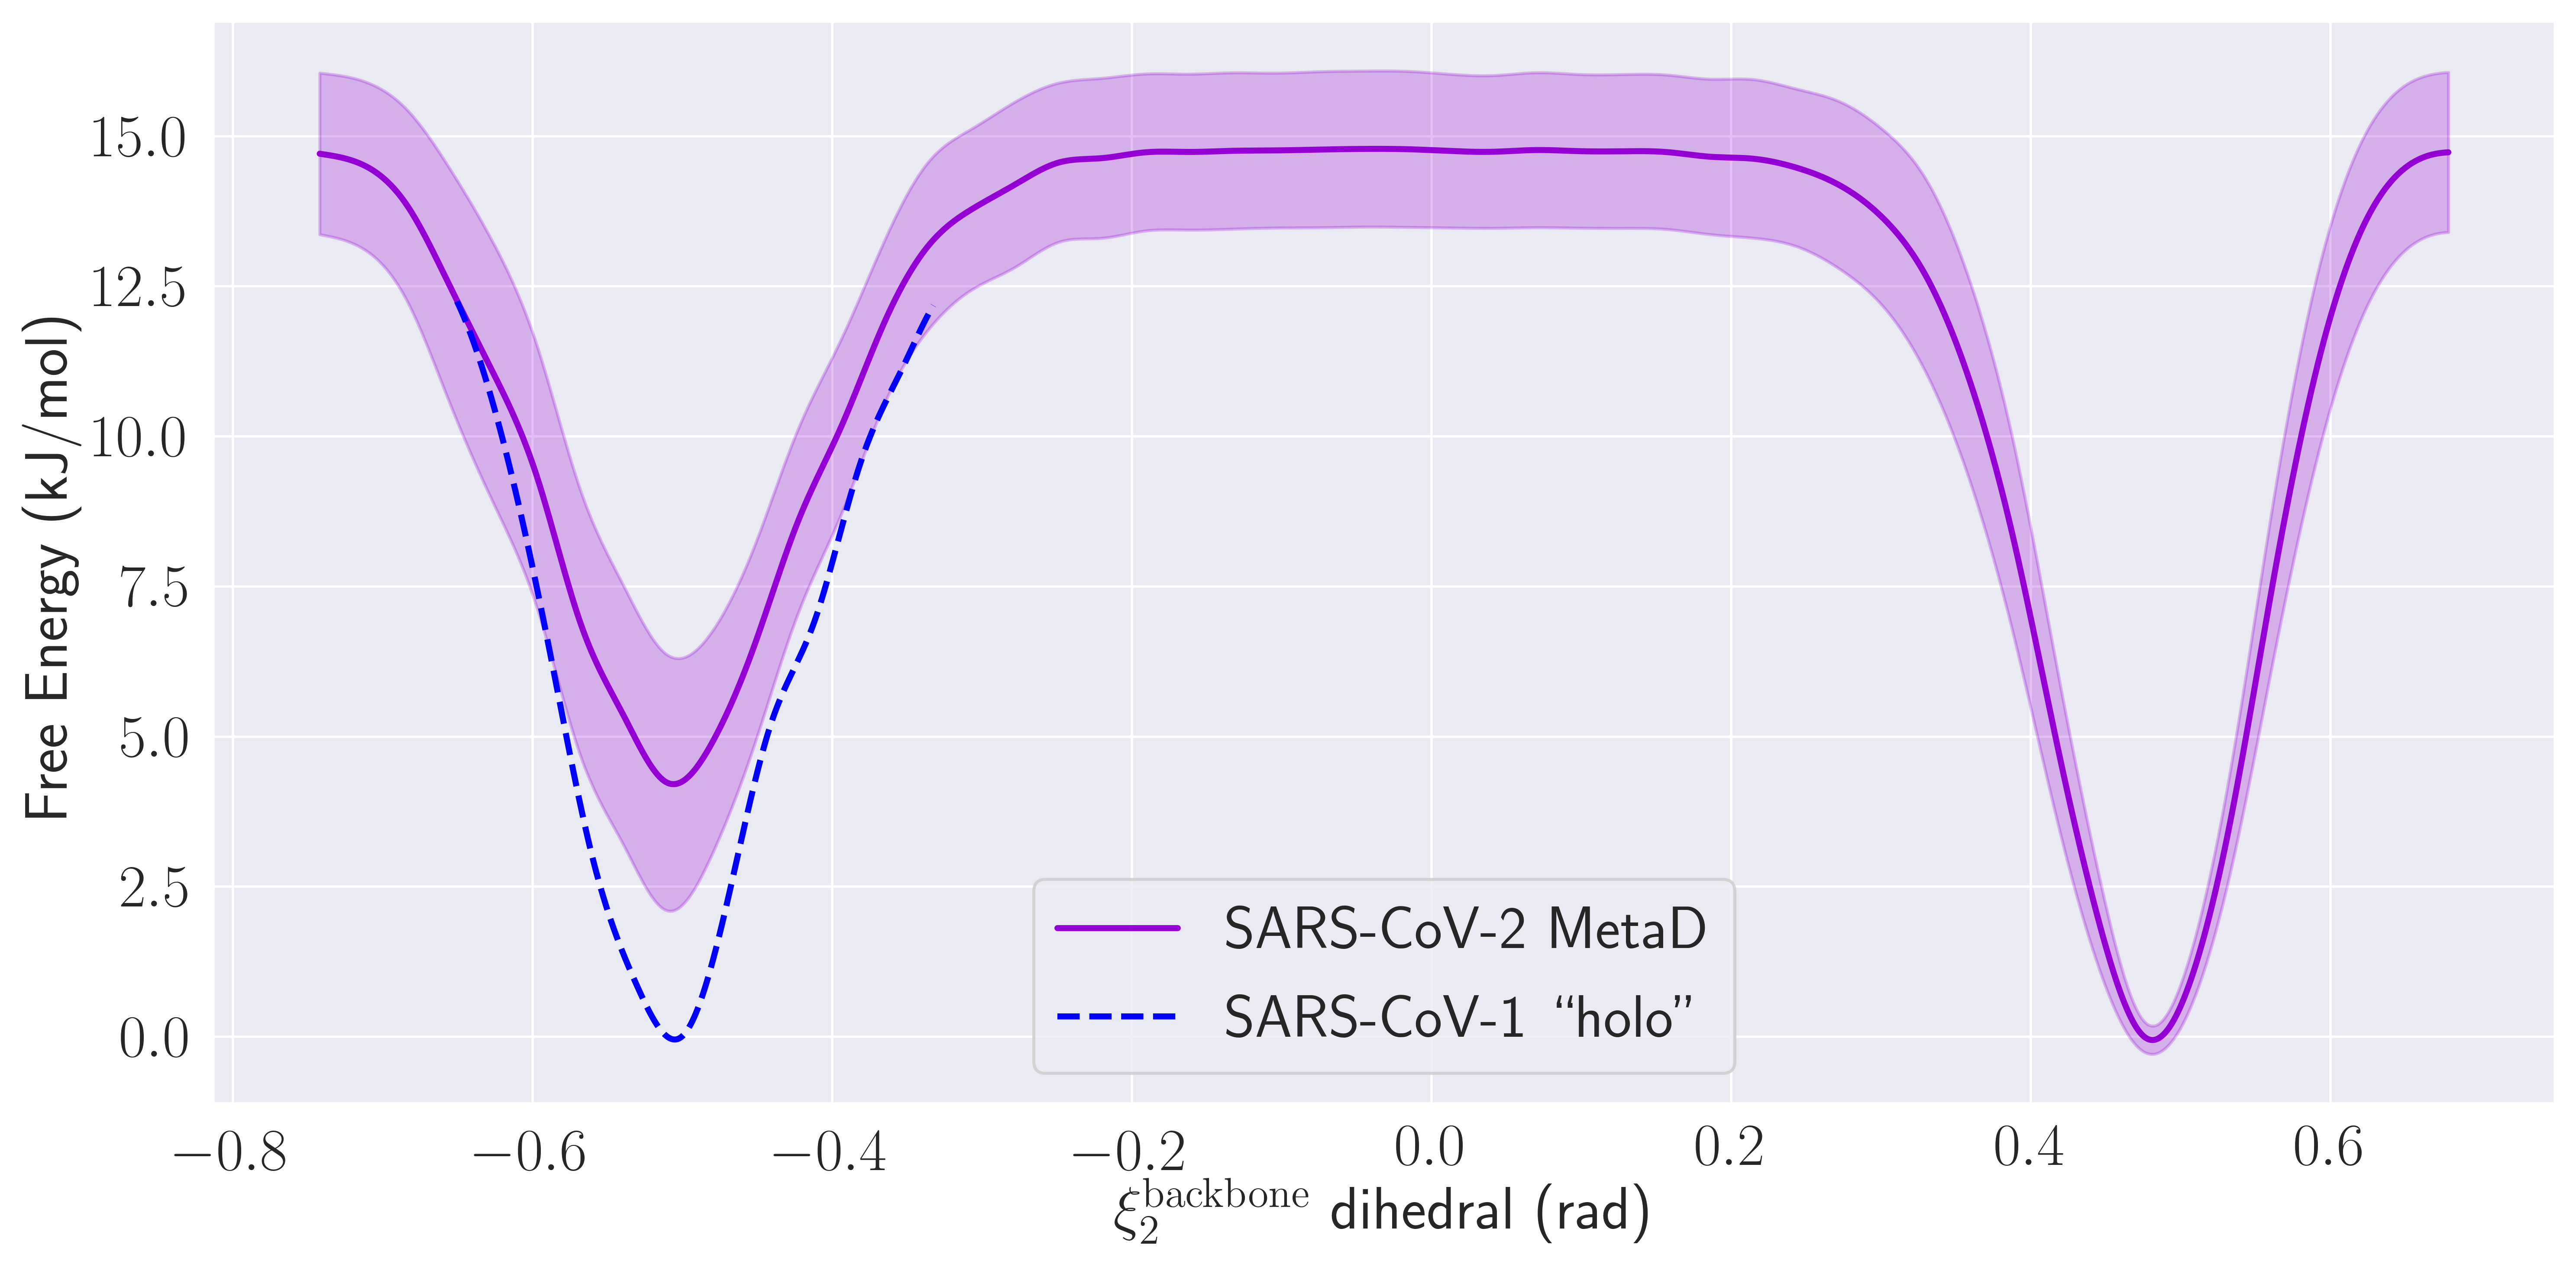
\includegraphics[width=\linewidth]{1DDih2FES_4Reps.png}
    \caption{Mean free energy surface obtained from the MD simulation of D3F-SARS-CoV-1 ``holo" (blue) and four replicas of His41 torsional MetaD simulations (purple), defined within the \dihtwo dihedral space. The shaded region corresponds to the standard deviation about each free energy point calculated over the set of MetaD replicas.}
    \label{fig:1DPMFAll_Dihtwo}
\end{figure}
%
%--------------------------------------
%
%
%
%               METHODS
%
%
%
%--------------------------------------
\section{Methods}

\subsection{Molecular Dynamics}
All MD simulations were performed in GROMACS version 2019.4 on the ARCHER Cray XC30 supercomputer on a single 2.7 GHz, 12-core E5-2697 v2 (Ivy Bridge) series processor node, NVIDIA GeForce RTX 2060 or GeForce GTX1080Ti GPUs with the CUDA 10.2 toolkit.  The AMBER14SB forcefield \cite{amberff14SB} was used to model the system, where ligand molecule forcefield parameters were generated using the General Amber ForceField v2 (GAFF2) with charges calculated using the AM1-BCC semi-empirical method.\cite{amber16}.\\

The structure of the candidate ligand LIG was derived from a virtual fragment expansion, docking, and screening exercise provided by Gabriel Grand, Elana Simon, Michael Bower, Bruce Clapham and Jonah Kallenbach of Reverie Labs.\cite{gabereverie} Protein X-Ray diffraction (XRD) structures for SARS-CoV-1  holo structure (PDB code: 2GZ7) \cite{2gz7} and SARS-CoV-2  apo structure (PDB code: 5RE4) were used for these simulations. Missing residues from the SARS-CoV-2 XRD structure were modelled using MODELLER \cite{modeller} and subsequently solvated in a 90 cubic box of TIP3P water molecules. \\

For co-solvent MD simulations, five of the candidate ligand (LIG) were placed in random coordinates within the box and the system net charge was neutralised by adding 4 sodium ions into the system. The co-solvent MD simulations was performed for 100 ns. The simulation of D3F bound in SARS-CoV-1  was performed for 10 ns. The net charge in the system was neutralised by adding 3 sodium ions. In all structures prepared for simulation, the His41 side chain was maintained at the N1-H tautomeric state, as this state is primed for nucleophillic attack from the Cys145 mercaptan in the active catalytic dyad.\\

The system was relaxed energetically using steepest-descent energy minimisation for 50000 steps with an energetic step size of 0.01 kJ/mol. The minimisation was terminated after the maximum energetic contribution was lower than a threshold of 10.0 kJ/mol. NVT and NPT equilibration was performed for 1 ns using two separate velocity-rescaling thermostat coupling temperature to velocities for protein, drug and solvent molecules (NVT), where a temperature of 300 K was maintained and 1 bar using the Parrinello-Rahman barostat (NPT).\cite{parrinello1981polymorphic} The Verlet cut-off scheme was employed to generate pair lists and the electrostatic interactions were calculated using the Particle-Mesh Ewald algorithm.\cite{pme} Both electrostatic and van der Waals interactions were cut off beyond 1.2 nm. All bonds involving hydrogen atoms were constrained using the LINCS algorithm.\cite{hess1997lincs} Production simulations ran with an integration stepsize of 2 fs. MDAnalysis was used to postprocess the MD trajectories for analysis.\cite{mdanalysis1, mdanalysis2}\\

\subsection{Metadynamics}
Four independent replicas of the non-tempered MetaD simulation were run to convergence.\cite{metaD} The bias potential was setup to sample energetically hindered rotations about the \dihtwo dihedral of His41 by biasing the sampling along the \dihone torsional profile directly. The bias was accumulated with a Gaussian deposition rate $\tau = 1$ ps. The deposited Gaussians had a fixed height of 0.1 kJ/mol and employed an adaptive width scheme in which the correlation between the biased CV space and the microscopic configuration space is utilised to recalculate the covariance matrix. A correlation length of 0.5 was used.\cite{adaptive} MetaD simulations were performed using Plumed 2.5.4.\cite{plumed}. All the data and Plumed input files required to reproduce the results reported in this paper are available on PLUMED-NEST (www.plumed-nest.org), the public repository of the PLUMED consortium \cite{plumed}, as plumID:20.027. 
%--------------------------------------
%
%
%
%               CONCLUSIONS
%
%
%
%--------------------------------------
\section{Conclusions}
We have presented the application of metadynamics to molecular dynamics simulations of the SARS-CoV-2  to better inform the drug discovery efforts including virtual screening, molecular docking and unbiased molecular dynamics simulations. We show that the proteolytic mechanism of  is contingent on the integrity of the His41-Cys145 catalytic dyad and that the rotation of the His41 imidazole side chain to Cys145 acts as an allosteric trigger to regulating this proteolytic activity.\\

Using metadynamics, we find that promoting ligand binding and sampling of the active site of the protease is achieved through disrupting the catalytic dyad by biasing over the His41 \dihone dihedral to subsequently sample over the \dihtwo dihedral. Using the (Cys145-$S_{\gamma}$)-(His41-N{$\epsilon$}) distance and the \dihtwo dihedral to define the collective variable (CV) space, we identify clusters of unbound, intermediary and bound conformations of the flexible  active site throughout the simulation. We show that repeated replicas of the His41 torsional metadynamics reproduce the free energy surface along the 1D \dihone and \dihtwo spaces. Our results detail the allosteric regulation of the SARS-CoV-2 \!\!, irrespective of the choice of ligand. The candidate ligand LIG acts as a toy model and its inadequacy in disrupting the catalytic dyad was established by drawing comparisons of its interaction in the  active site against the ligand D3F with SARS-CoV-1 \!\!.\\

The application of our analysis uncovers the changes on the receptor structure as a result of an allosteric mechanism resolved using enhanced sampling. This observation can assist in selecting an optimal strategy for screening ligands from drug libraries. The free energy comparison between the D3F unbound and bound ``holo" state minima suggests that the energy expended in disrupting the dyad can be readily recovered using ligand interactions in the active site, and so this open dyad state should be considered alongside the closed state as a target for virtual screening. We provide coordinates for structures corresponding to the open catalytic dyad state of SARS-CoV-2  as supplementary data for use in further studies. 
